\documentclass[a4paper,12pt]{report}
\usepackage{setspace}
\usepackage{rotating}
\usepackage{relsize}
\usepackage{graphicx}
\usepackage{pgfplots}
\usepackage{tikz}
\usetikzlibrary{calc}
\usetikzlibrary{trees}
\usepackage{float}
\usepackage{commath}
\usepackage{geometry}
\usepackage{listings}
\usepackage{booktabs}
\usepackage[toc,page]{appendix}
\usepackage[toc,acronym]{glossaries}
\usepackage[utf8]{inputenc}

% Set the overall layout of the tree
\tikzstyle{level 1}=[level distance=3.5cm, sibling distance=3.5cm]
\tikzstyle{level 2}=[level distance=3.5cm, sibling distance=2cm]

% Define styles for bags and leafs
\tikzstyle{bag} = [text width=4em, text centered]
\tikzstyle{end} = [circle, minimum width=3pt,fill, inner sep=0pt]

\definecolor{mygreen}{rgb}{0,0.6,0}
\definecolor{mygray}{rgb}{0.5,0.5,0.5}
\definecolor{mymauve}{rgb}{0.58,0,0.82}

\lstset{
  backgroundcolor=\color{white},   % choose the background color
  basicstyle=\footnotesize,        % size of fonts used for the code
  breaklines=true,                 % automatic line breaking only at whitespace
  captionpos=b,                    % sets the caption-position to bottom
  commentstyle=\color{mygreen},    % comment style
  escapeinside={\%*}{*)},          % if you want to add LaTeX within your code
  keywordstyle=\color{blue},       % keyword style
  stringstyle=\color{mymauve},     % string literal style
  numbers=left,					   % add line numbering
  numberstyle=\footnotesize,		   % set numbering styel
  stepnumber=1,					   % set numbering increment
  language=Java					   % set langauges
}

\newcommand{\nocontentsline}[3]{}
\newcommand{\tocless}[2]{\bgroup\let\addcontentsline=\nocontentsline#1{#2}\egroup}

\makeglossaries

\newglossaryentry{congstats}
{
        name=CONGSTATS,
        description={is a software product, part of a development contract in which the thesis was conceptualized. Its goal is to supply a statistical analysis tool for engineers examine traffic data}
}
\newglossaryentry{evaltool}
{
        name=evaluation tool,
        description={is part of the CONGSTATS service and was adapted and expanded for the usage in this thesis. It handles the analysis of processed \acrshort{fcd} data, congestion detection, incident matching and exports the analysis data}
}
\newglossaryentry{speedmatrix}
{
        name=Speed Matrix,
        description={is the data format of the processed \acrshort{fcd} data is a two-dimensional integer matrix representing a non-Euclidean time to road link space with the corresponding mean cell speed as value. The time dimension referrers to the 3-minute time increment of the day and the space dimension to the road link of the covered route of the speed matrix.}
}
\newglossaryentry{jam}
{
        name=congestion,
        plural=jams,
        description={ \textbf{or jam} is the spatial and timely accumulations of traffic participants, which leads to a reduction of travel speed and therefore reduction of traffic throughput. Because the plural of the noun congestion is not clearly recognizable, in the context of multiple congestion, the term \glspl{jam} will be used. A more detailed definition of a congestion can be found in chapter \ref{definition_congestion}}
}
	
\newacronym{adac}{ADAC}{Allgemeine Deutsche Automobil-Club e. V.}	 
\newacronym{tsm}{TSM}{Transportation System Management}
\newacronym{atdm}{ATDM}{Active Traffic and Demand Management}
\newacronym{atis}{ATIS}{Advanced Traveler Information System}
\newacronym{fcd}{FCD}{Floating Car Data}
\newacronym{fco}{FCO}{Floating Car Observer}
\newacronym{csv}{CSV}{Comma-seperated Values}
\newacronym{gsm}{GSM}{Global System for Mobile Communications}
\newacronym{umts}{UMTS}{Universal Mobile Telecommunications System}
\newacronym{lte}{LTE}{Long Term Evolution}
\newacronym{arbis}{ArbIS}{Arbeitstellenintegrationsystem}
\newacronym{ari}{ARI}{Autofahrer Rundfunk Information}
\newacronym{baysis}{BAYSIS}{Bayerische Straßeninformationssystem}
\newacronym{fpd}{FPD}{Floating Phone Data}
\newacronym{rtti}{RTTI}{Real Time Traffic Information}
\newacronym{tmc}{TMC}{Traffic Messaging Channel}
\newacronym{xfcd}{XFCD}{Extended Floating Car Data}
\newacronym{zvm}{ZVM}{Zentralstelle Verkehrsmanagement}
\newacronym{gps}{GPS}{Global Postioning System}

\onehalfspacing
\begin{document}
\showthe\textwidth
%418.25368pt.
%l.92 \showthe\textwidth

%\pagenumbering{roman}
% Title page goes first
\title{MASTER'S THESIS\\
[1cm]
\smaller Analysis of correlations between traffic data depended congestion detection and incident causalities}
% TODO red mal mit deinen Betreuern über den Titel, ob der so passt. ich glaube depended (abhängend) macht mehr sinn wenn es dependent (abhängig) heisst 
\author{
B. Sc. Jakob Erpf\\ 
[1cm]
\small Mentoring:\\ 
\small M. Eng. Barbara Karl (TUM)\\ 
\small Dr. - Ing. Matthias Spangler (TUM)\\ 
\small Dipl. - Ing. Stefan Gürtler (S\&W)\\
\small Dipl. - Ing. Johannes Grötsch (LBD)
}
\date{\today}
\maketitle

% Empty page for layout purpose
\clearpage

% Topic description is mandatory
\renewcommand\abstractname{Topic}
\abstract{}
Date of issue: 2020-05-04\newline
Date of submission:	2020-12-11\newline
\newline
The \gls{congstats} service is a statistical analysis tool, developed by the Munich office of SCHLOTHAUER \& WAUER GmbH and the thesis writer for the road administration of north and south Bavaria, to request and analyze traffic data. The traffic data used in this service is based on \acrfull{fcd}, provided by the Bavarian road administration. The aim of the service is to provide statistical monitoring and report functionalities on the traffic situation on freeway and state street network, to identify congestion-prone areas.

An interesting aspect of this congestion analysis is the correlation of congestion events and incidents. What are the circumstances leading to congestion in cause of an incident? What are the dependencies on an occurred incident, for example roadworks or accidents? The knowledge on the impact of roadworks on the traffic flow or which accidents lead to traffic capacity reductions could improve traffic management and incident response actions. The question of how the congestions represented by the \acrshort{fcd} correlate with actual traffic incidents and their causalities, will be evaluated in this thesis. 

To answer this research question, the writer is provided with datasets containing \acrshort{fcd} and traffic incident data. The \acrfull{zvm} provides the incident’s reports, which hold statistics on the traffic incident situation and detailed reports for the specific incidents.

These datasets then are processed and analyzed for possible correlations between detected congestions in the \acrshort{fcd} and the reported incidents from the \acrshort{zvm}. Therefore scope of the thesis consists of the following tasks:

\begin{itemize}
  \item review of the available data and information
  \item definition data characteristics and indicators
  \item definition and implementation of a methodology for detecting jams in \acrshort{fcd}
  \item definition and implementation of a methodology for analyzing the correlation between congestion and incident events
  \item interpretation of the results
\end{itemize}

The student will present intermediate results to the mentors 
		(Barbara Karl, M.Eng.: TUM-VT; 
		Dr.-Ing. Matthias Spangler: TUM-VT; 
		Dipl.-Ing. Stefan Gürtler: Schlothauer \& Wauer; 
		Dipl.-Ing. (FH) Johannes Grötsch: ZVM) 
	in the fifth, tenth, 15th and 20th week.

The student must hold a 20-minute presentation with a subsequent discussion at the most two months after the submission of the thesis. The presentation will be considered in the final grade in cases where the thesis itself cannot be clearly evaluated.

% Disclaimers
\renewcommand\abstractname{Preliminary information and disclaimers}
\abstract{
%TODO Datennutzungserklärung
}

% Germany abstract
\renewcommand\abstractname{Kurzfassung}
\abstract{Deutsche Fassung des 'Abstracts'}

% Englisch abstract
\renewcommand\abstractname{Abstract}
\abstract{Current navigation systems often use accumulation strategies to estimate travel time while considering time delays through congestions, which are based on analyzing the history of the time delays on the considered street network. This approach can be disturbed through uncommon events creating short time blockages or be biased through regular accruing, long-term traffic volume reductions. This thesis evaluates a new idea of predicting time delays and accident probability through analyzing the correlation of congestions and incidents which are placed in timely and spatial vicinity of each other. To evaluate this, three real world datasets from the year 2019 will be considered. After an algorithmic approach to analyzing a derivative of a floating car dataset for congestions and locating spatial and timely adjacent incidents from the Bavarian street information systems, the thesis will evaluate if and how these incidents and \glspl{jam} are correlated with each other. To further give an idea of how such statistical data could be used, the thesis will elaborate on the possibility and plausibility of using correlation statistics for \gls{jam} and/or incident prediction.}

%\setcounter{secnumdepth}{3}
%\setcounter{tocdepth}{3}\
\addtocontents{toc}{\protect\thispagestyle{empty}}
\tableofcontents % TODO fix no page number in TOC
\thispagestyle{empty}

\chapter{Introduction}
\pagenumbering{arabic}
\setcounter{page}{1}
Traffic \glspl{jam} are a known problem to everyone, ever attempting to begin the summer season with a car trip on the first day of the summer break. When the number of road users increases or the capacity of the road way decrease du to various reasons, a demand-supply imbalance is created \cite{Tang2019}. This impacts passenger traffic as well as transportation of goods through blocked bottlenecks and decreased travel speeds. They lead to unreliable travel times, inefficient usage of resources, and an increase in emissions, like pollutants or noise \cite{FHA2011}. Another effect is a decrease in road safety, due to high driver tempers or inattentive mind, which can result in higher accident counts \cite{Sun2016}. This induce enormous social costs due to billions of hours lost in \glspl{jam} and induced mental stress. \cite{RetallackOstendorf2019,BardtFritsch2014,ADAC2019}

It is therefore essential to reduce risks of \glspl{jam}, as well as accidents, with an increased understanding of the traffic accident causes, trigger effects of \glspl{jam} and roadwork consequences, to maintain a fluent traffic flow and traffic safety. Tailored \acrfull{tsm} strategies, focused on automatic reactions for significant traffic event, could enable \acrfull{atdm} of high traffic demands in reduced traffic volume areas \cite{Tang2019}. This would go towards reducing the economic, environmental, and social costs associated with accidents, roadworks or \glspl{jam}. Part of this \acrshort{tsm} strategies implemented in a \acrshort{atdm} system, could be a form of traffic incident prediction systems, with the potential to identify compromising conditions in real-time, allowing according to actions to be taken to avoid consecutive events. \cite{RetallackOstendorf2019} 

\bigskip

This thesis approaches \gls{jam} and incident prediction by evaluating the statistical relation of \glspl{jam} and incidents to predict the chance of a consecutive event. These consecutive events can be \glspl{jam}, as well as incidents. Depending on the severity of an accident, \glspl{jam} can be provoked. The other way round, \glspl{jam} can facilitate accidents due to the change of traffic flow. Another scenario are construction sites and maintenance which can also lead to both \glspl{jam} and accidents, because of the reduction of traffic volume, changes in road guidance, or other modifications to the normal traffic situation. Although the scope of the thesis does not cover the specifics on a complete production system for \gls{jam} and accident detection, prediction and response, it will take the concept of such a system and focus the possibility of predicting such events, which then would make the development of such a system possible. 

A system capable of the described mentioned functionalities would likely consist of the following processing components.

\begin{itemize}
  \item Data acquisition for congestion and incident detection
  \item Data analysis for the finding the probabilities of consecutive events
  \item Concept for traffic management and controlling responses
\end{itemize}

The first component, in charge of detecting \glspl{jam} as well as incident, requires input data like speed, volume, occupancy to represent the traffic situation and incident reports to define incident characteristics. The next component would then analyze the resulting dataset to find characteristic features of the congestions and incident, which will be determined in this thesis. In the case the analysis of the characteristic shows a possible and imminent event it would trigger the last component to initiate appropriate controlling actions and prepare incident responses.

In the following chapters of this introduction section, the reader will be introduced to the concepts and systems used to cover the input and output requirements in this thesis.

\section{Continuous Floating Data}

To detect \glspl{jam}, continuous data about the speed or movement of the vehicle on the road is necessary. This kind of information can be collected through a variety of different systems, to represent a real-time or at least current picture of the traffic situation. 

The current street network of Bavaria heavily depends on stationary sensors, to assess the traffic situation. This includes inductive loops, infrared or radar detectors, which can provide traffic indicators like volume, speed, time gaps, jams, density and many others. The data collected with just stationary sensors can only describe the traffic trends restricted to their location and coverage, which requires complex simulations and modeling to aggregate data for the missing areas where there is no sufficient coverage. Adding to this is the fluctuating result set quality which depends on the input data and simulation model quality. Especially highways are equipped with stationary sensor, but the lower index streets network is only covered by a fragmented net of detectors with distances of up to 100\,km between detectors \cite{INDRIX2015}. Fortunately, nowadays cars as well as drivers and riders are equipped with technology that allows real time tracking and comprehensive data collection. Cars can gather information from the build in sensors as well as an on-board GPS and mobile devices from drivers and riders can also be used to collect location and movement data. \cite{Randelhoff2016}

\acrfull{fcd} is continuously collected during the usage of a car by the on-board GPS and represents the individual movements. Typical this incorporates the coordinates, timestamp, road section, course and routing data points. These are regularly sent to a central FCD unit/service via mobile radio communication (\acrshort{gsm}-, \acrshort{umts}- or \acrshort{lte}-based), to be aggregated and combined with stationary data to an area wide picture of the traffic situation. In this form they can be used for traffic analysis and management. \cite{Randelhoff2016,LAPID2020}

A derivative of \acrshort{fcd} is \acrfull{xfcd}, developed by BMW. It expands the collection of data points of an \acrshort{fcd} with data from the vehicle sensors and systems like breaks, rain sensors, driver assistance systems and more. These data points add a number of analytic opportunities to generate a more precise and detailed traffic picture. \cite{LAPID2020}

In contrast to \acrshort{fcd}, \acrlong{fpd} does not need an on-board GPS or car systems to create movement data but assumes that driver’s and rider’s mobile devices will register and deregister at the radio tower along the road. \acrshort{fpd} uses this registration information to determine the radio cell the phone is currently in, how long is stayed in that cell and tracks the devices when switching to another cell or tower. It is therefore able to collect a much larger quantity of datasets but lacks the accuracy of \acrshort{fcd} which transmit the GPS location of the car itself. That been said, on roads with a high coverage of radio tower like in urban areas or on highways, \acrshort{fpd} is able to achieve a comparable accuracy. Mobile service providers collect this anonymized \acrshort{fpd} and forward them to a traffic management unit, which can analyze the date for disturbances and give feedback through the traffic information channels. \cite{Randelhoff2016,LAPID2020}

Another type of floating data type is \acrfull{fco}. \acrshort{fco} does not only collect its own \acrshort{fcd} but also data about its surroundings with the built-in sensors. This includes the automatic recognition of cross- or opposite traffic, traffic volume or relative speeds to other cars. This additional data not only add detail, but also allow for correctional fusion algorithms to reduce uncertainties or errors in the pure \acrshort{fcd}. \cite{Randelhoff2016}

\section{Street Information Systems}

Besides of having a real-time or current picture of the traffic situation, the concept of the thesis also relies on information about current disturbances or possible triggers of disturbances. 

\subsubsection{\acrfull{baysis}}
For disturbances in the form of accidents the \acrfull{baysis}, a publicly available information system from the Bavarian street administration, will be used. The systems task is the acquisition, collection and analysis of street network related information, which contains infrastructure inventory and condition, traffic volumes and other key values, as well as an accident register with detailed reports. An export of this accident register with detailed reports is provided by the \acrshort{zvm} for this thesis.

\subsubsection{\acrfull{arbis}}
Another type of disturbance to consider is roadworks, for which an export from the \acrfull{arbis}, a software tool and database used by the Bavarian infrastructure ministry, will be consulted. The system is used to collect and archive all current, planned and passed roadwork and maintenance projects on the Bavarian state street net-work. With the collected information from \acrshort{arbis}, an effective, economic and safe execution of roadworks can be achieved. Furthermore \acrshort{arbis} can provide detailed report exports about current projects to the Bavarian traffic information office and traffic information channels. \cite{trafficon2017}

\section{Traffic Status Information}

To deliver information from traffic management systems to the road users traffic messaging channels can be used. Three examples are \acrfull{rtti}, \acrfull{tmc} and \acrfull{atis}.

The \acrshort{tmc} is a messenger system for congestions and other traffic incidents. The public available service is free to use and publishes current congestion notifications in compatible navigation system and announcements in the local radio channels. In the scope of the \acrshort{tmc} the road network is split into \acrshort{tmc} sections. These sections are used to define the spatial location of the incident to report and typical start / end with road linkups. More detailed Incident information is obtained from the police or reports from traffic participants which adds a considerable before publication delay. It is therefore spatial and temporal to rather imprecise. \cite{LAPID2020}

Another traffic information source is the \acrshort{rtti}. \acrshort{rtti} supplies traffic participants with information about current events or suggested diversions like \acrfull{tmc}, but with a much spatial higher accuracy. Through a \textit{Geocast}, which is expansion of a multicast with a geolocation, the spatial precision of the \acrshort{rtti} is superior to the \acrshort{tmc}. This \textit{Geocast} can be either a geometrical address like a GSM84 coordinate or a symbolic address, reaching a spatial accuracy of up 100m.  \cite{LAPID2020,HindenDeering2006,ImielinskiNavas1996}. This is why \acrshort{rtti} is the industry standard of suppling vehicle and third party navigation system with up to date traffic information. Another difference to \acrshort{tmc} is the accessibility. Unlike the publicly available \acrshort{tmc}, \acrshort{rtti} is vendor specific and most time payed service, like BMWs ConnectedDrive \cite{BMW2020}. 

% TODO more infos and literature to TMC / Geocasts
% https://ec.europa.eu/transport/themes/its/road/action_plan/traffic-information_en
% https://www.itwissen.info/RTTI-realtime-traffic-information.html
% https://ieeexplore.ieee.org/document/861224

The most up-to-date variation of a traffic status information system is the \acrfull{atis}, such as GoogleMaps, HERE or Waze. Like \acrshort{rtti} is it a provider based service, but mostly without costs and less device constraint. Because of these missing accessibility constraints and the fact that in current times nearly 70\% of people carry a smartphone \cite{IZM2020}, the user base of such services is quite substantial. This does not invalidate the usage of \acrshort{rtti} and \acrshort{tmc}, since there are present in most separate and built-in navigational systems, but rather makes \acrshort{atis} a considerable alternative. With the added benefit of being able to not only publish information about the traffic situation, but also collect variations of \acrshort{fcd}, \acrshort{atis} is the most promising technology for \acrshort{atdm} and \acrshort{fcd} collection. 

\bigskip

In the scope of this thesis only a selection of these introduced data collection systems will be further relevant. 
\begin{itemize}
  \item \acrshort{fcd} for the congestion data
  \item \acrshort{baysis} and \acrshort{arbis} for incident data
  \item \acrshort{atis} for the concept of \acrshort{atdm}
\end{itemize}

\chapter{Objects of Research}
	This chapter defines the key terms which will be referenced to during the thesis.
\section{Incident}
		Incidents in the scope of this thesis, an incident can be accidents, as well as ongoing roadwork or maintenance on the Bavarian street network. These are also the events, which the concept of the thesis tries to predict through the analysis of the correlation of said incidents to jams.
	\subsubsection{Accident}
		An accident is an unexpected and unintentional traffic event, that typical results in damages, injuries and reduction of traffic volumes. These events can be triggered a number of different reasons, where in this thesis we a mostly interested in the trigger of slow, congested traffic or roadworks.
	\subsubsection{Roadwork}
		As roadwork classify all static and moving construction sites, as well as temporary blockages or disturbance due to snow clearing, road maintenance and alike. 
	
\section{Congestion}
\label{definition_congestion}

\paragraph{Naming} The noun congestion does not have clear plural, which is why in the case of multiple congestion, the term jams will be used. These two terms are seen as interchangeable for their reference to a single or multiple congestion events.

\subsection{Descriptive}

Jams or a single congestion in layman terms are spatial and timely accumulations of traffic participants, resulting in speeds slower or sometimes much slower than free flow. In severe cases this is also often described a stop-and-go or stopped traffic. They are triggered by a reduction of traffic throughput in volume or an increase of traffic demand. Studies have shown that these triggers are usually caused by four categories of disturbances. \cite{TRB2003,FHA2011}

\subsubsection{Traffic-Influencing Events}

\begin{itemize}
	\item Incidents : Events that disrupt the normal free flow of traffic, like vehicular crashes, breakdowns or debris. These physical obstacles block lanes or hard shoulders, forcing other road user to execute evasive maneuver and deviate from their normal path. This ultimately changes driving behavior, reduces the quality of traffic flow and traveling speed. Even when incidents are not directly on the roadway they can impact the traffic flow due to emergency responses create blockades or ineffective driving behavior of traffic participants gapping on the incident.
	\item Roadwork : Managed and unmanaged construction sites on the roadway that result in physical changes to the highway environment. This includes a reduction of lanes, lane diversion, elimination of hard shoulders or road closures, which reduce the road capacity and reduce travel speeds.
	\item Weather : Changes in environmental conditions like, heavy rain or snow fall can negatively impact driver behavior. The reduction of visibility will usually result in a reduction of traveling speeds and increase of headway. This reduces the overall capacity of the highway. Bright sunlight, smoke or icy road surfaces lead so a similar effect.
\end{itemize}

\subsubsection{Traffic Demand}

\begin{itemize}
	\item Fluctuations in Normal Traffic : Variations in demand in day-to-day traffic volumes can overload systems with fixed capacities. This can result in travel speed reductions without any specifically occurring event.
	\item Special Events : Special cases where events drastically change the demand in their vicinity and overload the system. As with incidents, off-road events can affect driving behavior due to visual distractions and change the traffic-flow. 
\end{itemize}

\subsubsection{Physical Highway Features}

\begin{itemize}
	\item Traffic Control Devices : Poorly time or defective traffic signals, ineffectively controlling the traffic flow, contribute to the creation of jams and travel time reductions.
	\item Physical Bottlenecks or Capacity : The capacity of a road is mostly dependent on the number of lanes and shoulder, as well as the alignment (curves and grades). Physical changes on the road environment like in merging areas, tool booths or road endings reduce the capacity and therefore promote the formation of jams. The road capacity can also be influenced by the driving behavior, which heavily depend on the familiarity of the roadway to the driver. Drivers familiar with routinely congested tend to reduce their headway and therefore increase the capacity \cite{Charlton2013}.
\end{itemize}

\subsubsection{Driving-behaviour}
As above-mentioned, driving behavior can influence the traffic flow as well as capacity and is mostly influenced by environment and the familiarity of the road. Research showed that driving on familiar road has a negative effect on safety aspects of driving behaviors, like in-attentional blindness for roadside features \cite{Charlton2013}. Another decreasing factor is the state-of-mind, better know as rage-driven or aggressive driving, resulting in rapid lane changing, cross cutting or passing on shoulders \cite{Shinar2004}. This can lead to driving behaviors where drivers don't keep up smooth accelerations, but rather break suddenly or accelerate in rapidly, other vehicles need to react accordingly. This creates a chain reaction leading to reduced travel speed. These are called "phantom jams" because they do not have any specific origin and are common in high density traffic regions, like cities and high demand highways. \cite{ASTRA2020} 

\bigskip

This general layman's definition of jams is essential correct, but not sufficient for the data scientific approach in this thesis. The Bavarian ministry for streets does not have an official definition at the time of writing and there is no unified definition or thresholds when reduced speed or time delays can classify data as a congested or slow. This makes it necessary to form a specific definition of \glspl{jam} and their speed/space/time thresholds, for the scope of this thesis. For instance the \acrshort{adac} classifies highway traffic moving with mean speed lower than 20 km/h as jammed \cite{ADAC2019}. In Switzerland the ministry for streets has a more severe definition with a mean speed under 10 km/h \cite{ASTRA2020}. A definition just this available literature does not consider the data is would be applied on. Therefore the representation of the speeds occurring in jams from the FCD dataset, introduced in chapter \ref{dataset_fcd}, should be adducted to further tailor a definition to our needs. 

\subsection{Data scientific}

\begin{figure}[h]
	\centering
	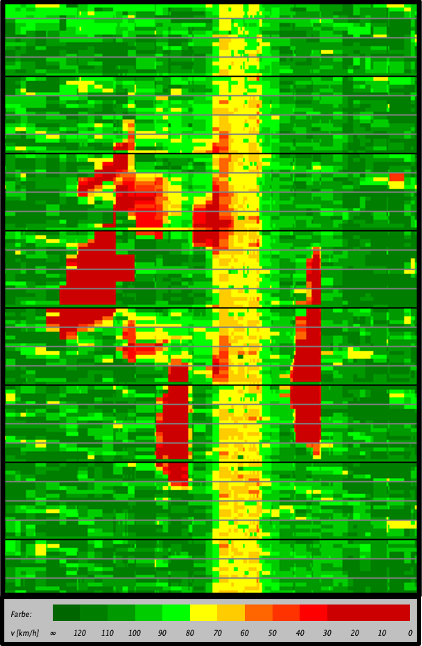
\includegraphics[scale=0.8]{./assets/SpeedMatrixPlot_single}
	\caption{Speed matrix plots of FCD data, showing a scattered cluster}
	\label{img:speedMatrixPlot_singleCluster}
\end{figure}

Figure \ref{img:speedMatrixPlot_singleCluster} shows a section of a random speed matrix plot from the FCD dataset, containing a scattered congestion cluster. The horizontal and vertical extend represents the spatial and temporal location of each cell. The color of the cell indicated the mean absolute speed recorded in the time frame and on the link of the cell (detailed gradient is shown in the legend of \ref{img:speedMatrixPlot_singleCluster}).

The visual representation show that a congestion mostly contains speed of less than 30 km/h, shown in \textit{dark red}. A closer look on the cluster in the top left reveals that speed around 40-50 km/h, shown in \textit{lighter red} tones, may be also considered, to incorporate the complete congestion area. Speeds above at least 50 km/h, starting with the \textit{orange/yellow} categories, should not be included in the definition, because it would classify regular speed limits, represented by the broad vertical \textit{orange/yellow} stripe, as jammed traffic. This makes two speed threshold for jammed and slow-moving traffic necessary adequately detecting congestion clusters. With this information and some learning during calibration of the clustering algorithm (see section \ref{cluster_calibration}) the following thresholds for the jammed and slow speed, classifying \glspl{jam} in FCD data where defined.

\begin{itemize}
	\item Speed threshold for jammed state : $v_{crit,jammed} = 30 \frac{km}{h}$
	\item Speed threshold for slow-moving state : $v_{crit,slow} = 60 \frac{km}{h}$
\end{itemize}

To exclude cell errors and discard detections, too small to have to be considered as jams, the length and duration is used for filtering. 

\begin{itemize}
	\item Minimum length of a congestion : $l_{min} = 1000 m$
	\item Minimum duration of a congestion : $t_{min} = 9 min$
\end{itemize}

If $l < l_{min}$ or $t < t_{min}$ is given, $l$ being the maximum spatial extend and $t$ being the maximum temporal extend, the detection should be ignored.

\chapter{Correlation}
\label{definition_correlation}
This chapter will explain the later used statical methods and their mathematical definitions. This is to provide an in depth understand how the results presented in later chapter are where comprised. This also helps to clarify which methods and assumptions implemented to handle a mixed data-based analysis.

\bigskip

Correlation is an analysis procedure that measures the correlation coefficient, which represents the degree of linear, bivariant, monotonic or other kind of relation, which could also be described as the degree of association between two variables \cite{HerzSchlicherSiegener1992}. In most statistics the following common types of can be found: Pearson's $r$, Kendall's $\tau$, Spearman  $\rho$ or the Point-Biserial correlation \cite{Ramzai2020,SPSS2020a,SPSS2020b}. Besides off these, there are many more correlation coefficients which varying in they applicability and interpretability. Depending on which type of data variables are to be analyzed, it it necessary to choose an applicable correlation coefficient. The type of data variable and relation combination are the most restricting features for choosing a suitable correlation coefficient. 

\section{Variable Types}
\label{correlation_variable_types}
Data variables can be grouped into continuous and categorical, depending what kind of observation they describe. Variables are considered to be continuous, also know as quantitative, when relating to measurements like speed, distance or age, which can take on an unlimited number of values between the lowest and highest points of measurement \cite{McCue2007}. These continuous variables can be separated into two subsets. 

\begin{itemize}
	\item \textbf{Interval} variables can be measured along a continuum and have a numerical value. \cite{Laerd2020}
    \item \textbf{Ratio} variables are interval variables, with the added condition that the values is zero if there is no measurement for this value. \cite{Laerd2020}
\end{itemize}

Categorical variables on the other hand are limited in the number of values, referring to a category, rank or choice, like a vehicle type or Yes/No answers. These categorical variables can be separated into three subsets.

\begin{itemize}
	\item \textbf{Nominal} variables have two or more categories, but with no intrinsic order. \cite{Laerd2020}
	\item \textbf{Dichotomous} are nominal variables which have only two categories or levels. \cite{Laerd2020}
    \item \textbf{Ordinal} are nominal variables that have two or more categories and are ordered or ranked. \cite{Laerd2020}
\end{itemize}

The datasets to be examined in this thesis include continuous variables of the type interval, as well as all three types of categorical variables (see \ref{dataset_baysis} and \ref{dataset_arbis}).

\section{Coefficient Types}
\label{correlation_coefficient_types}
The datasets from \acrshort{baysis}, \acrshort{arbis} (see section \ref{dataset_baysis}, \ref{dataset_arbis}) as well as the generated data includes continuous, as well as categorical variables, describing interval, nominal, dichotomous and ordinal characteristics. For an exact analysis of relations between these characteristic the appropriate correlation coefficient suited for the apparent variables needs to be chosen. This task in itself is quite complex due to the number of coefficients to evaluate, amount of literature, numerous assumptions and the many disagreements in the field of statistics. From a comprehensive literature review the following correlation coefficients and tests, prominent in current studies and papers where selected, in dependency of their suitability for the apparent relation.

For a flattened introduction into correlation statistic, the article from Jun Ye \cite{Yun2020} is highly recommended. % https://junye0798.com/post/everythin-you-need-to-know-about-correlation/

\subsection{Continuous - Continuous}
\label{correlation_pearson}

As stated in \ref{correlation_variable_types} continuous variables are metric measurements in the form or distances or durations. The most common correlation coefficient for continuous variables is the non-parametric Pearson's $r$.

\subsubsection{Pearson's $r$}

% https://statistikguru.de/spss/produkt-moment-korrelation/pearson-korrelation-in-spss.html

Pearson's $r$ describes the linear correlation of such continuous, non-ranked variables and does not assume normality or a normal distributed sample set as it is non-paramteric. It is therefore suitable for the examination of continuous-continuous variable relations, where we can assume finite size of variance and covariance. \cite{BenestyChenHuang2009,Sulthan2018}
 
The general correlation coefficient, shown in equation \ref{formula_correlation_basic} is the foundation for deducing Pearson's $r$. It is defined by the fraction of the covariance (see equation \ref{formula_correlation_covariant}) of two vectors $x$ / $y$ of length $i$ / $j$ and their standard deviation (see equation \ref{formula_correlation_deviation}).\cite{HerzSchlicherSiegener1992}

\smallskip

\begin{equation}
\label{formula_correlation_basic}
	\rho = \frac{\sigma_{xy}}{\sigma_{x}\sigma_{y}}
\end{equation}

\begin{equation}
\label{formula_correlation_covariant}
	\sigma_{xy} = \sum_{ij}(x_i-\mu_X)(y_n-\mu_Y) \cdot p(x_i,y_j)
\end{equation}

\begin{equation}
\label{formula_correlation_deviation}
	\sigma_{x,y} = \sum_{i}(x_i,y_i-\mu_{x,y})^2 \cdot p_i
\end{equation}

\bigskip

The equation \ref{formula_pearson} shows Pearson's correlation coefficient $r$, which is a direct usage of the definition in \ref{formula_correlation_basic}, assuming that both data variables have the same length, named $i$. The symbols $\bar{x}$ and $\bar{y}$ correspond to the means of the data variabel $x$ and $y$, respectively. \cite{BenestyChenHuang2009,Zychlinski2018}

\smallskip

\begin{equation}
\label{formula_pearson}	
	r_{xy} =  \frac{\sum_{i}{(x_i-\bar{x})(y_i-\bar{y})}}{\sqrt{\sum_{i}{(x_i-\bar{x})^2}\sum_{i}{(y_i-\bar{y})^2}}}
\end{equation}

\bigskip

The equation can simplified to \ref{formula_pearson_simplified} with the $SS$ corresponding to the summed squares and $SP$ corresponding to summed products.

\smallskip

\begin{equation}
\label{formula_pearson_simplified}
	r =  \frac{SP_{xy}}{\sqrt{SS_x}{SS_y}}
\end{equation}

\subsubsection{Interpretation of $r$}
Pearson's $r$ can have values of the range $-1$ to $+1$. If one variable moves in the same direction as the other, it is called positive correlation, represented by a positive correlation coefficient. In the case of one variable moving in a positive direction, when a second variable is moving in a negative direction, the correlation is called negative and has a negative coefficient. Another characteristic is the ration of change in the variables. When both variables change at the same ratio, they are linearly correlated. When both variables do not change in the same ratio, then they are non-linearly or curvi-linear correlated. 

\subsubsection{Interpretation of $|r|$}
The degree of correlation, also be described as strength of association, is also called effect size and shows how strong the two variables are related with each other. It is defined by the absolute values of $r$ (or any other correlation coefficient), mathematical written as $|r|$. According to Cohen \cite{Cohen1988} the effect size of each correlation coefficient falls into one of two categorizes $D$ and $R$. $D$ corresponds to coefficients utilizing the mean difference and standardized mean difference. He defined the values of $D$ coefficients as small $D$ = .20, medium $D$ = .50, and large $D$ = .80 \cite{Piegorsch2002}. The group of $R$ coefficients includes measures based on variance \cite{Walker2005}. Cohen propose vastly different values of .01, .06, and .14 serve as indicators of small, medium, and large effect sizes for the $R$ group \cite{Cohen1988}. However, if these values fit the purpose of the analysis, depends on the underlying data and is at discretion of the researcher.

% http://www.leeds.ac.uk/educol/documents/00002182.htm
% https://www.psychometrica.de/effect_size.html
% https://www.cedu.niu.edu/~walker/personal/Walker%20Kendall's%20Tau.pdf

According to Cohen recommendations for mean-based coefficents \cite{Cohen1988,Piegorsch2002,Walker2005} and with consideration of the guidelines of Wolfe \cite{Wolfe2017} and Regber \cite{Regber2016} following rules are defined for the interpretation of the effect size of $r$.

\begin{itemize}
  \item When both variables change in the same ratio, the absolute value is 1.0, which is called perfect correlation.
  \item If the range is above .80, it is called high degree of correlation.
  \item A moderate degree of correlation lays in the range of .50 to .80.
  \item When range is between .30 to .50, it is called low degree of correlation.
  \item When it is lower than .30, it shows that there is no correlation, which can be called absence of correlation.
\end{itemize}	

\subsubsection{Significance of $r$}
To determine if $r$, is statically significant, a chi-square test can be applied to find the $p$-value, testing the probability of independence. Equation \ref{formula_chi_squared_simplified} shows the chi-squared statistic taken from Wikipedia, cited from Karl Pearson \cite{Pearson1990}.

\smallskip

%\begin{equation}
%\label{formula_chi_squared}	
%	\chi^2 = \sum_{i=1}^{m}{\frac{(N_i-n_{0i})^2}{n_{0i}}}
%\end{equation}

\begin{equation}
\label{formula_chi_squared_simplified}	
	\chi^2 = \sum_{i=1}^{n}{\frac{(O_i-E_i)^2}{E_i}} == N\sum_{i=1}^{n}{\frac{(O_i/N-p_i)^2}{p_i}}
\end{equation}

\begin{itemize}
	\setlength\itemsep{0.1em}	
	\item[] $N$ is the total number of data samples 
	\item[] $O_i$ is the number of data samples with type $i$
	\item[] $E_i = N p_i$ is the expected number of data samples with type $i$
\end{itemize}

The $p$-value can be comprised by comparing $\chi^2$ to a $\chi^2$-distribution by calculation or by using a conversion table \cite{Piegorsch2002}, with the degree of freedom $df = (n_x - 1) \cdot (n_y - 1)$. The resulting  $p$-value, is compared to the significance level $\alpha$, to either accept ($p > \alpha$) or reject ($p <= \alpha$) the null hypothesis ("The means are equal to the population"). For a 2-tailed $p$-value, $p$ will be doubled to incorporate both ends of the distribution. Usually a value of $0.05$ is chosen for $\alpha$, which means that there is a 5\% risk of falsely rejecting the null hypothesis. From this definition the following two interpretations of the correlation coefficient can be drawn. \cite{OTSD2020}

\begin{itemize}
	\item $p <= \alpha$ means that the null hypothesis can be rejected and indicates that is a significant dependency between the two tested variables. It can be concluded that the increase or decrease of one variabel does significantly related to the increase or decrease of the other.
	\item $p > \alpha$ means that there is \textbf{no} significant dependency between the two variables and no conclusion can be drawn for the correlation.
\end{itemize}

\subsection{Continuous - Nominal}
This type of relation is objectively the most complex to evaluate. One well known method to analyze the relation between a continuous and categorical variable, which is not ranked and has more than to values, is the analysis of variance (ANOVA). As it is a parametric test it unfortunately assumes normal or gaussian distributed variables, which is not give in our datasets (see chapter \ref{data}). A non parametric approach of the ANOVA is the rather uncommon Kruskal-Wallis H-test \cite{Leon1998}. Both tests indicates if at least one variabel stochastically dominates another, but not in which groups or in how many groups this domination occurs \cite{OTSD2020}. They therefore do not provide a statement about the correlation strength, but the statistical significance of a possible correlation.

The research of a correlation coefficient for the relation of a continuous and nominal variable only provided the eta ($\eta$) coefficient from Pearson \cite{Benninghaus2007}. 

\subsubsection{Eta ($\eta$) coefficient}
% https://stackoverflow.com/questions/52083501/how-to-compute-correlation-ratio-or-eta-in-python/52084418
The $\eta$ coefficient, also called correlation ratio (used as $\eta^2$), measures the relationship between variables based on the sums of squares used in the ANOVA \cite{Lewis2012,Benninghaus2007}. More concrete, $\eta$ is the squared root of ratio between $SS_x$ and $SS_y$ \cite{Shaldehi2013}.

\smallskip
\begin{equation}
\label{formula_eta}	
	\eta = \sqrt{\frac{SS_x}{SS_y}}
\end{equation}

As the data doesn't fit the parametric requirements of ANOVA, the non-parametric Kruskal-Wallis H-test, shown in equation \ref{formula_kruskal_wallis}, will be used to test for variance.

% https://de.wikipedia.org/wiki/Kruskal-Wallis-Test
% https://www.sciencedirect.com/topics/nursing-and-health-professions/kruskal-wallis-test
\smallskip
\begin{equation}
\label{formula_kruskal_wallis}	
	H = \frac{12}{n(n+1)}\sum_{h}{\frac{S_h^2}{n_h}}-3(n+1)
\end{equation}

\subsubsection{Interpretation of $\eta$}
The coefficient can have values in the range from $0$ to $1$. The effect size of $\eta$, which can be categorized in the $R$ group, can be interpreted as follows \cite{Regber2016,Cohen1988}.

\begin{itemize}
	\item $\eta <= .06$ : The correlation strength is weak
	\item $.06 < \eta < .14$ : A moderate strength of correlation
	\item $\eta >= .14$ : There is a strong correlation
\end{itemize}

For the Kruskal-Wallis H-test applies the following. The higher value of $H$, the higher the variance between the variables. The significance of $H$ must be tested with $\chi^2$.

\subsubsection{Significance of $\eta$}
The significancy evaluation for the $\eta$ coefficient is done via the $p$-value of the Kruskal-Wallis H-test, which is calculated with the chi-squared test ($\chi^2$), defined in sub section \textit{Significance of $r$} in \ref{correlation_pearson} \cite{Filipiak2013}.

\subsection{Continuous - Dichotomous}
The Point Biserial correlation is a special form of the Pearson's $r$ correlation coefficient and suited to evaluate the association of continuous-dichotomous relations. 

\subsubsection{Point Biserial}
The Point Biserial notation, shown in formula \ref{formula_point_biserial}, can be derived from Person's $r$ with the assumption of $y$ only taking dichotomy values of 0 and 1, so that $\bar{y} = p$. The distinction of the cases

\begin{itemize}
	\item $i \cdot p$ referring to $y=1$ an with $1 - p = q$ bigger than $\bar{y}$
	\item $i \cdot q$ referring to $y=0$ an with $1 - p = -p$ smaller than $\bar{y}$
\end{itemize}
allow to form \ref{formula_point_biserial_from_pearson} from \ref{formula_pearson}, which can be simplified to \ref{formula_point_biserial}. \cite{Tate1954,CohenWest2003,Bortz2004,DeJesus2019}

\smallskip

\begin{equation}
\label{formula_point_biserial_from_pearson}
	r_{pq} =  \frac{n \cdot p (\bar{x}_{y=1}-\bar{x}) \cdot q + n \cdot p (\bar{x}_{y=0}-\bar{x}) \cdot (-q)}{\sqrt{\sum_{i}{(x_i-\bar{x})^2} \cdot (n \cdot p \cdot q^2 + n \cdot q \cdot (-p)^2)}}
\end{equation}
%\begin{equation}
%\label{formula_point_biserial_from_pearson_simplyfied}
%	r_{pqi} =  \frac{n \cdot p \cdot q \cdot (\bar{x}_{y=1}-\bar{x}_{y=0})}{\sqrt{\sum_{i}{(x_i-\bar{x})^2} \cdot (n \cdot p \cdot q)}}
%\end{equation}
\begin{equation}
\label{formula_point_biserial}
	r_{pq} =  \frac{\bar{x}_{y=1}-\bar{x}_{y=0}}{\sqrt{\sum_{i}{(x_i-\bar{x})^2}}} \cdot \sqrt{n \cdot p \cdot q \cdot} 
\end{equation}

\smallskip

It must be pointed out that if the dichotomous variable is artificially binarized, i.e. there is likely continuous data underlying it, biserial correlation is a more a measurement of similarity instead of association.

% https://de.wikipedia.org/wiki/Wilcoxon-Mann-Whitney-Test
% https://pythonfordatascienceorg.wordpress.com/wilcoxon-sign-ranked-test-python/
%The Wilcoxon signed-rank test is the non-parametric univariate test which is an alternative to the dependent t-test. It also is called the Wilcoxon T test, most commonly so when the statistic value is reported as a T value. Which scipy.stats.wilcoxon() uses for it’s calculation. This is the recommended test to use when the data violates the assumption of normality. It’s used to test if there is a significant difference on scores when there is a “before” and “after” condition of some treatment or intervention. An example of this is if you where to collect the blood pressure for an individual before and after some treatment, condition, or time point.
%
%The hypothesis being test is:
%
%Null hypothesis (H0): The difference between the pairs follows a symmetric distribution around zero.
%Alternative hypothesis (HA): The difference between the pairs does not follow a symmetric distribution around zero.
%If the p-value is less than what is tested at, most commonly 0.05, one can reject the null hypothesis.

\subsubsection{Interpretation of $r_{pq}$}
Due to the mathematical similarity of the Point Biserial to the Pearson's $r$, the general interpretation of Pearson's $r$ can be applied to Point Biserial with some adjustments. According to Cohen \cite{Cohen1988} the following can be used as guidelines for the effect size $r_{pq}$ \cite{Leblanc2017}.

\begin{itemize}
	\item $r_{pq} <= \pm \: .10$ : The correlation strength is weak
	\item $\: .30 < r_{pq} < \: .50$ : A moderate strength of correlation
	\item $r_{pq} >= \: .50$ : There is a strong correlation
\end{itemize}

\subsubsection{Significance of $r_{pq}$}
The significancy evaluation of the Point Biserial coefficient is done via the 2-tailed $p$-value, a doubled chi-square test (see sub section \textit{Significance of $r$} in \ref{correlation_pearson}).

\subsection{Continuous - Ordinal}
For ordinal variables, also called ranked or rank ordered, the commonly used Spearman's $\rho$ can be applied, but should be replaced by Kendall's $\tau$ because of it superiority over Spearman \cite{Newson2002}. 

\subsubsection{Kendall's $\tau$}
Kendalls $\tau$ evaluates the order of rank pairs, instead of the squared rank difference, which make is more robust against outliners. Because we can assume that the data has ties implemented, the $\tau$ with ties must be used. The general definition is shown in equation \ref{formula_kendalls_r}, with $P$ referring to the \textit{proversion} and $I$ to the \textit{inversion}. With the assumption that the continuous measurement $x$ is or can be ordered, the ordinal/ranked variable $y$ will be wrongly ordered. After forming all possible rank pairs between $x$ and $y$, $P$ and $I$ can be deduced and $\tau$ can be calculated. \cite{Reiter2015,Bossart2017}

\begin{itemize}	
	\item[] \textbf{Proversion} ($+$) is the number if pairs, where $x < y$ 
	\item[] \textbf{Inversion} ($-$) is the number of pairs, where $x > y$ 
	\item[] \textbf{Ties} ($0$) are pairs where $x = y$
\end{itemize}

\begin{equation}
\label{formula_kendalls_r}
	\tau = \frac{P-I}{\sqrt{(\frac{n(n-1)}{2}-T_x) \cdot (\frac{n(n-1)}{2}-T_y)}}
\end{equation}
\begin{equation}
\label{formula_kendalls_r}
	T_x = \sum_{i=1}^n \frac{t_{x_i}(t_{x_i}-1)}{2}
\end{equation}
\begin{equation}
\label{formula_kendalls_r}
	T_y = \sum_{j=1}^m \frac{t_{y_j}(t_{y_j}-1)}{2}
\end{equation}
\smallskip

\begin{itemize}
	\setlength\itemsep{0.1em}	
	\item[] $N$ is the total number of rank pairs 
	\item[] $P | I$ are the pro- and inversion of pairs
	\item[] $T_x | T_y$ are the ties in $x$ and $y$
	\item[] $n | m$ are the number of rank bindings in $x$ and $y$
	\item[] $t_{x_i} | t_{x_i}$ are the length of rank bindings in $x$ and $y$
\end{itemize}

\bigskip

Thought transformation we can simplify the general definition to equation \ref{formula_kendalls_r} \cite{Reiter2015}.

\begin{equation}
\label{formula_kendalls_r}
	\tau = \frac{P-I}{\sqrt{(P+I+T_x) \cdot (P+I+T_y)}}
\end{equation}

\subsubsection{Interpretation of $\tau$}
% https://www.reddit.com/r/AskStatistics/comments/44ypc4/kendall_taus_effect_size_question/
Strictly speaking, Kendall's $\tau$ is not a measure of effect size, like Pearson's $r$, but tends to be of similar magnitude. Because of this similarity the general interpretation defined in the sub section \textit{Interpretation of effect size $|r|$} in \ref{correlation_pearson} can be applied. To adapt the guidelines to the lesser sensitivity of $\tau$, they are scaled downwards \cite{Regber2016}.

\begin{itemize}
	\item $\tau <= \pm \: .10$ : The correlation strength is weak
	\item $\: .30 < \tau < \: .50$ : A moderate strength of correlation
	\item $\tau >= \: .50$ : There is a strong correlation
\end{itemize}

\subsubsection{Significance}
The significancy evaluation of Kendall's $\tau$ coefficient is done via the 2-tailed $p$-value, elaborated in sub section \textit{Significance of $r$} in \ref{correlation_pearson}.

\subsection{Categorical - Categorical}
The Pearson's $\chi^2$ test from section \ref{correlation_pearson} can also be applied to categorical data for independence statistics. Two correlation coefficients using $\chi^2$ are Cramer’s $V$ and Theil’s $U$. Both can be used to analyze categorical-categorical relations, but differ in the type of result they provide \cite{OutsideTwoStandardDeviations2018}. Cramer’s $V$ is a symmetric measure, providing us with a measure of association strength. Theil’s $U$, the uncertainty coefficient, on the other hand is a conditional measure and represents the predictability of an association \cite{Akoglu2018,StackExchange2020}. Because the Theil’s $U$ measurement of predictability provides a better interpretability, it is the preferred  result choice for the interpretation and implementation. 

\subsubsection{Cramer’s V}

Cramer’s V, also called Cramer's phi ($\Phi_c$), is a measurement for the relation of two nominal variables. In equation \ref{formula_cramers_v_biased}, showing the notation of Cramer’s $V$, $k$ and $r$ are the number of columns and row, respectively. $\varphi$, the phi coefficient, is defined by $\frac{{\chi^2}}{n_{ij}}$. The $\chi^2$ shown in \ref{formula_cramers_v_chi} is derived from equation \ref{formula_chi_squared_simplified} with the expansion to columns an rows. \cite{Sheskin1997,Bergsma2013}
\smallskip
\begin{equation}
\label{formula_cramers_v_biased}
	V = \Phi_c =  \sqrt{\frac{{\varphi^2}}{min(k-1,r-1)}} = \sqrt{\frac{\frac{{\chi^2}}{n_{ij}}}{min(k-1,r-1)}}
\end{equation}
\begin{equation}
\label{formula_cramers_v_chi}
	\chi^2 =  \sum_{i,j}{\frac{(n_{ij}-\frac{n_i n_j}{n})^2}{\frac{n_i n_j}{n}}}
\end{equation}

\smallskip

The above notation of $\Phi_c$ can be heavily biased, trending to overestimate the strength of relation. It can be corrected with \ref{formula_cramers_v_corrected}, using the corrected notation \ref{formula_cramers_v_phi_corrected} for $\tilde{\varphi^2}$ and \ref{formula_cramers_v_k_corrected} as well as \ref{formula_cramers_v_k_corrected} for $k,r$. \cite{Bergsma2013}
\smallskip
\begin{equation}
\label{formula_cramers_v_corrected}
	\tilde{V} = \tilde{\Phi_c} = \sqrt{\frac{\tilde{\varphi^2}}{min(\tilde{i_{max}}-1,\tilde{j_{max}}-1)}}
\end{equation}
\begin{equation}
\label{formula_cramers_v_phi_corrected}
	\tilde{\varphi^2} = max(0,\varphi^2 - \frac{(k-1)(r-1)}{n-1})
\end{equation}
\begin{equation}
\label{formula_cramers_v_k_corrected}
	\tilde{k} = k - \frac{(k-1)^2}{n-1}
\end{equation}
\begin{equation}
\label{formula_cramers_v_r_corrected}
	\tilde{r} = r - \frac{(r-1)^2}{n-1}
\end{equation}

\bigskip

\subsubsection{Theil’s U}
% https://rstudio-pubs-static.s3.amazonaws.com/558925_38b86f0530c9480fad4d029a4e4aea68.html
The uncertainty coefficient, also called entropy coefficient, is a measurement for the association between two nominal variables and in comparison to Cramers V, provides a much better predictability statement. It is based on the of concept of comparing the entropies of variables to determine a degree of association \cite{Hoang2019}. The entropy of a distribution (see equation \ref{formula_theils_hx}) and the conditional entropy (see equation \ref{formula_theils_hxy}) are used to calculate the uncertainty coefficient $U(X)$ \cite{Glen2017,Glen2018}, which tells us: given Y, what can fraction can be predicted for X \cite{Hoang2019}.

\smallskip
\begin{equation}
\label{formula_theils}
	U(X) = \frac{H(X)-H(X|Y)}{H(X)}
\end{equation}
\begin{equation}
\label{formula_theils_hx}
	H(X) = -\sum_{x} p_{X}(x)log p_X(x)
\end{equation}
\begin{equation}
\label{formula_theils_hxy}
	H(X) = -\sum_{x,y} p_{X,Y}(x,y)log p_{X,Y}(x,y)
\end{equation}

% Definition: Theil’s U symetrical
%\begin{equation}
%\label{formula_theils_sym}
%	U(X,Y) = \frac{H(X)U(X|Y)-H(Y)U(Y|X)}{H(X)+H()Y} = 2[\frac{H(X)+H(Y)-H(X|Y)}{H(X)+H(Y)}]
%\end{equation}

\subsubsection{Interpretation}
The Interpretation of Cramers $V$ and Theil's $U$ is similar to Pearson's correlation coefficient $r$, witha reduced range of $0$ to $1$ and a adapted scale of effect size according to \cite{Cohen1988} and \cite{Ellis2010}

\begin{itemize}
	\item $V|U <= \pm \: .10$ : The correlation strength is weak
	\item $\: .30 < V|U < \: .50$ : A moderate strength of correlation
	\item $V|U >= \: .50$ : There is a strong correlation
\end{itemize}

\subsubsection{Significance vs. Uncertainty}
\label{correlation_significance_uncertainty}

TODO: define the usage of significance vs uncertainty for Cramer's V and Theil's U
% TODO define the usage of significance vs uncertainty for Cramer's V and Theil's U
%https://de.statista.com/statistik/lexikon/definition/122/signifikanz/
%https://www.ncbi.nlm.nih.gov/pmc/articles/PMC3387884/
%https://www.ons.gov.uk/methodology/methodologytopicsandstatisticalconcepts/uncertaintyandhowwemeasureit
%https://www.ncbi.nlm.nih.gov/books/NBK459346/
%https://www.npr.org/sections/health-shots/2019/03/20/705191851/statisticians-call-to-arms-reject-significance-and-embrace-uncertainty?t=1600534742009
%https://www.tandfonline.com/doi/full/10.1080/00223131.2013.820155

\section{Correlation Matrix}

As a result we have the following correlation coefficients and statistical test to be used for the mixed analysis of continuous and categorical variables. These will be implemented into a processing script in section \ref{methodology_??}.

\bigskip

\begin{table}[ht]
	\centering
	\begin{tabular}{c|c|c}
					& Categorical 		& Continuous\\
		\\[-1em]
		\hline
		\\[-1em]
		 			& Cramer’s V  	& Eta $\eta$	\\
		Categorical	& Theil’s U		& Point Biserial\\
					& 				& Kendall's $\tau$\\
		\\[-1em]
		\hline
		\\[-1em]
					& Eta $\eta$		  			& \\
		Continuous	& Point Biserial		& Pearson's $r$\\
				& Kendall's $\tau$		& \\
	\end{tabular}
	\caption{\label{tab:table-name}Candidates of Correlation Coefficients}
\end{table}
	
\chapter{Data Foundation}
\label{data}
In this chapter the provided datasets from the previously mentioned street information systems and the FCD provider will be elaborated. First an overview of FCD in general and the available dataset is given. Then the incident datasets from BAYSIS and ArbIS are presented with descriptive statistic.

\section{FCD}
\label{dataset_fcd}
 
As described in chapter 1.1, \acrshort{fcd} represents the movement of vehicles and can be used to calculate vehicle speeds and trajectories. The provided dataset contains the aggregated absolute and relative speeds for the highways and state streets, calculated from \acrshort{fcd} data. The process of speeds estimation with \acrshort{fcd} data is explained in detail by Felix Rampe in chapter 4 of his thesis \textit{Traffic Speed Estimation and Prediction Using Floating Car Data} \cite{Rempe2018}, but is outside of the scope for this thesis. The FCD is mapped mapped onto the HERE \cite{HERE2020} network, to be compliant with the geolocation system used in the project.

% TODO add more info about FCD if there is time 
% https://athene-forschung.unibw.de/doc/127445/127445.pdf
% Traffic Speed Estimation and Prediction Using Floating Car Data.pdf

Each of these aggregated speeds represent the mean speed over a three minute time interval on the corresponding road section. This arrangement of speeds for each time step and space step is called speed matrix and is the base data for the congestion detection. Figure \ref{speedMatrixPlot_mutipleMixedClusters} shows a visual representation a speed matrixes with the horizontal axes being the spatial extend and the vertical axes the time extend. Deep greens represent free flowing traffic with ~130 km/h, which is the norm speed in Germany (in German called “Richtgeschwindigkeit”) on highways set the legislator. The speed scale then develops linearly downwards deep red indicating traffic with 30 km/h or less. 

\begin{figure}[h]
	\centering
	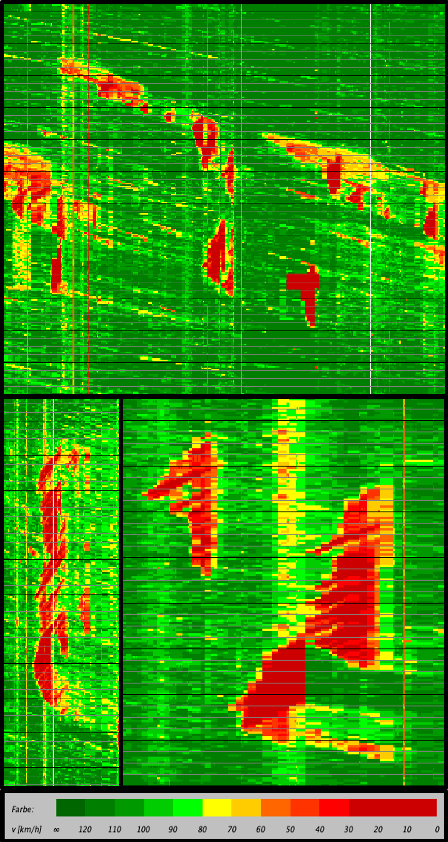
\includegraphics[scale=0.8]{./assets/SpeedMatrixPlot_mutiple}
	\caption{Speed matrix plots of processed FCD data, showing different jam clusters}
	\label{img:speedMatrixPlot_mutipleMixedClusters}
\end{figure}

The observer will clearly recognize the jams represented by the clusters of red and orange cells in the figure \ref{img:speedMatrixPlot_mutipleMixedClusters}, with the angled extends towards the right down edge, due to the vehicle trajectory through space and time. These cluster, also shown in the two lower pictures, which representing one or multiple jams can be densely packed or spotted into smaller clusters or, depending on the severity of a jam can be seen, by the cluster which contain more orange or yellow cells than red. 

From this visual clarity, the continuity of the data points and the precision on 3-minute intervals it can concluded that a comprehensive algorithmic approach should be able to detect such congestion events. This being said, the dataset does contain defects in the form of missing values for complete road sections, which can interfere with detection algorithm. Another defect type are obviously wrong speed block, meaning sudden speed drops or jumps to areas of identical speeds with an abnormal temporal and spatial extend, which have to be ignored during processing. 

\section{BAYSIS}
\label{dataset_baysis}

The \acrfull{baysis} as describe in chapter \ref{dataset_baysis}, collects a wide range of different information types, one of then being accidents with the corresponding police reports. Accidents have a strong traffic influence on the Bavarian street network, with more than 400.000 being recorded in the year 2019 (StMi, 2020), hence their importance in this topic. The provided export from BAYSIS contains all accidents of the year 2019 on the Bavarian highway network, which are 10262 records in number. 

Each accident report includes a variety of specifications, which covers environmental indicators like weather or light situation, accident characteristics like accident type, collision object or cause, as well as information over the involved like nationality, age and gender. In total, one report contains 132 values, describing the accident, participant and environment. Because we do not want to form a stereotype of accident participant but rather find significant accident characteristics or environmental factors most of the descriptive values for the involved persons are not considered. Variables without any values or single values are also neglected. To meet a statistical significant result a diverse distribution in the values would be preferred, to reduce the risk of uncertain relation. Because the correlation of a non distributed variable, which for example has one values occupying a 95\% major share, is based on a sample set comprised of mostly the same samples, the interpretability for a correlation to other values but the major share is very limited (see \ref{correlation_significance_uncertainty} for more detailed elaboration of this assumption).

From this curtailed pool of correlate able and analyze able characteristics all parameters that have a logical significance with causes or effects of an accident will be considered in the analysis. To give an overview about what results can be expected on the basis of the provided dataset the 15 most plausible relevant parameters of the dataset will be illustrated. The parameters are also categorized in the variable types, defined in chapter \ref{correlation_variable_types}. All mentioned diagrams are available as larger prints in the appendix \ref{appendix_baysis} for better readability. 

\begin{figure}[H]
	\centering
%	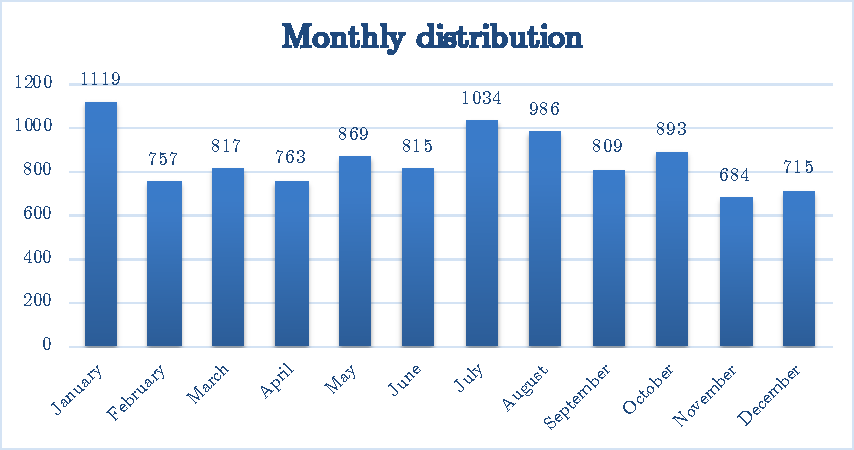
\includegraphics[scale=0.8]{./assets/baysis_dataset_monthly_absolute.pdf}
	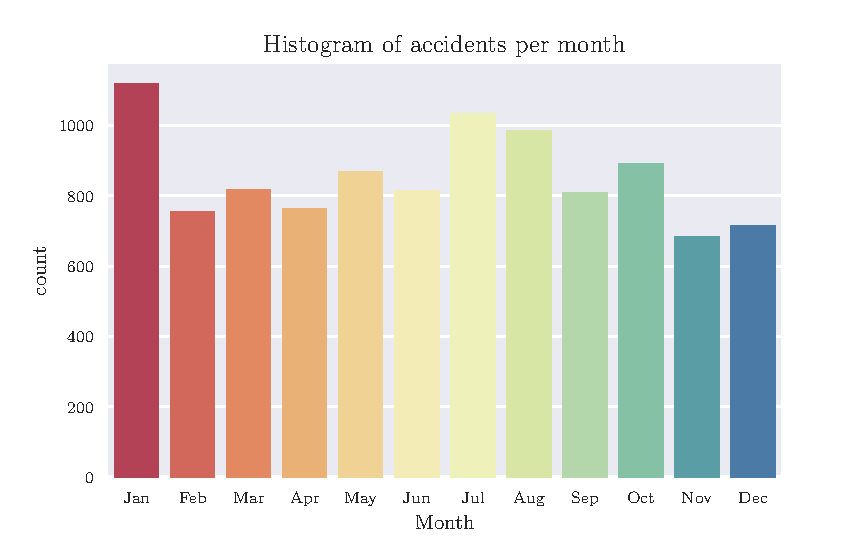
\includegraphics[scale=0.5]{../CorrAnalysis/data/BAYSIS/01_dataset/plots/baysis_dataset_hist_month}
	\caption{Monthly distribution of accident report counts}
	\label{img:baysis_monthlyDist_absolute}
\end{figure}

%\begin{figure}[h]
%	\centering
%	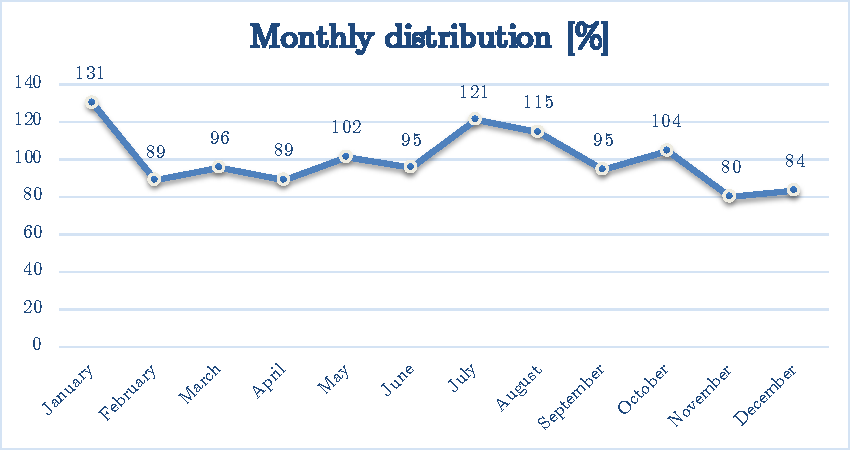
\includegraphics[scale=0.8]{./assets/baysis_dataset_monthly_percentage.pdf}
%	\caption{Monthly distributions of accident report counts in percentages to mean}
%	\label{img:baysis_monthlyDist_percentage}
%\end{figure}

A look on the monthly distribution of accidents recorded by BAYSIS (see figure \ref{img:baysis_monthlyDist_absolute}) shows that that the months of January,July and August have considerably higher number of accidents. The monthly distribution expressed in percentages (see figure \ref{img:baysis_monthlyDist_percentage}) supports this deviation with a respectively 31\%, 21\% and 15\% increase over the mean count of 855 accidents per month. The increased number in January can be explained with the increased number of accidents due to ice and snow conditions, which reduces traction on roads and can lead to uncontrollable vehicle behavior. Also the reduced visibility during snow falls increases accident numbers. In July and August the increased demand because of public holidays is the most probable explanation.

\begin{figure}[h]
	\centering
	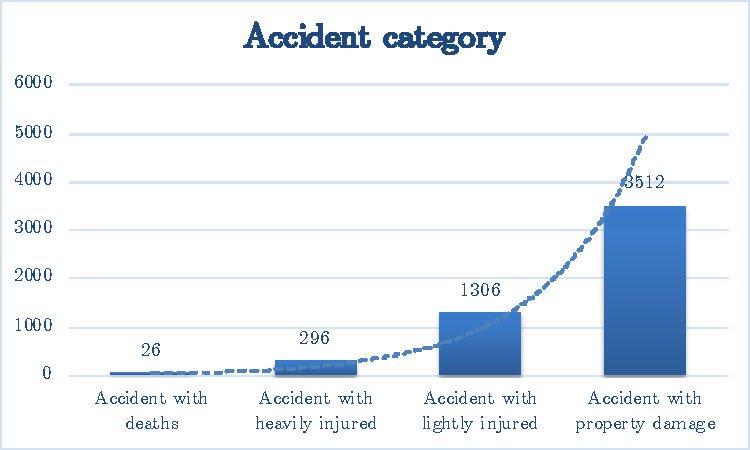
\includegraphics[scale=0.6]{./assets/baysis_dataset_Kat.pdf}
	\caption{Distribution of the accident category 'Kat'}
	\label{img:baysis_dataset_Kat}
\end{figure}

\paragraph{Kat}
The accident categories, described by the variable shown in figure \ref{img:baysis_dataset_Kat},  range from just accident with damaged property to deathly accidents, with the number of deadly accidents having the lowest count. The distribution also fits the exponentially trend line, which allows the statement that statistical deadly accidents are exponentially unlikely. The variable consists of four values, which can be considered as ordered, and is therefore ordinal.

\begin{itemize}
	\setlength\itemsep{0em}
	\item 0 = Kleinunfall
	\item 1 = Unfall mit Getöteten
	\item 2 = Unfall mit Schwerverletzten
	\item 3 = Unfall mit Leichtverletzten
	\item 7 = Unfall mit Sachschaden
\end{itemize}

\begin{figure}[h]
	\centering
	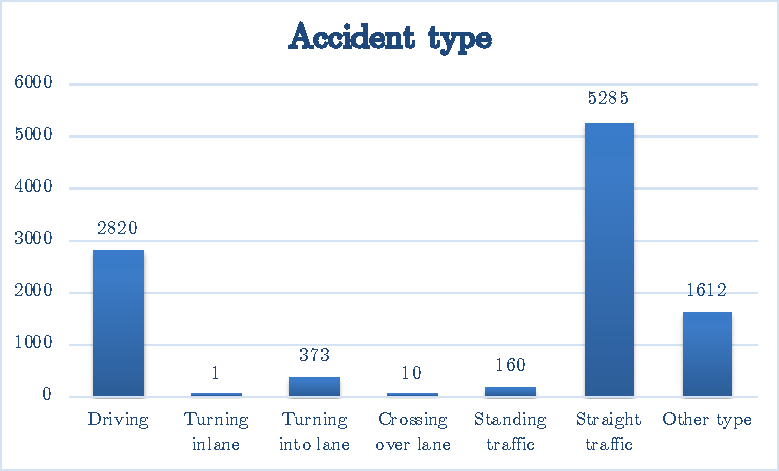
\includegraphics[scale=0.6]{./assets/baysis_dataset_Typ.pdf}
	\caption{Distribution of the accident type 'Typ'}
	\label{img:baysis_dataset_Typ}
\end{figure}

\paragraph{Typ}
The accident type variable (shown in figure \ref{img:baysis_dataset_Typ}) incorporates different kind of traffic movements, from straight and driving to turning movements. Beside of an 80\% share of accidents related to driving or straight driving situations, the parameter does not indicate any other features. The variable does not show any order and is therefore of nominal type.

\begin{figure}[H]
	\centering
	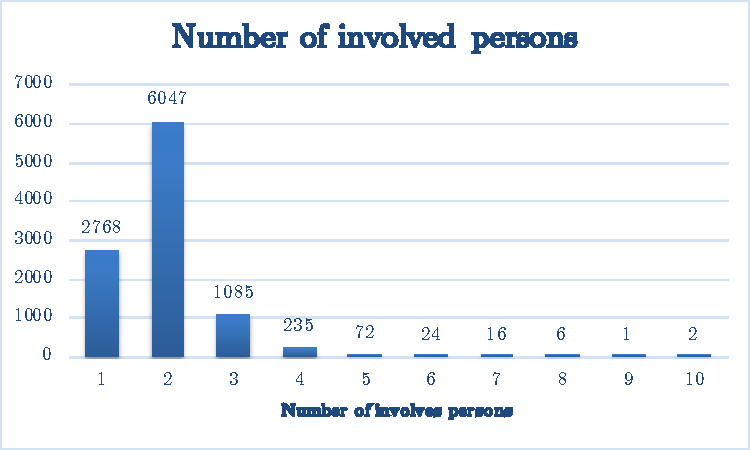
\includegraphics[scale=0.6]{./assets/baysis_dataset_Beteil.pdf}
	\caption{Distribution of the number of involves persons 'Beteil'}
	\label{img:baysis_dataset_Beteil}
\end{figure}

\paragraph{Beteil}
The distribution of the number of involved persons (shown in figure \ref{img:baysis_dataset_Beteil}) shows that more than 96\% of accidents have three or less involved persons. The major share of two involved persons makes up for 56\% and the second biggest of one involved person for 30\% of the total count. This also means the accidents with more than three involved persons are statistically insignificant. Because of the increasing order of values, the variable is of ordinal type.

\begin{figure}[h]
	\centering
	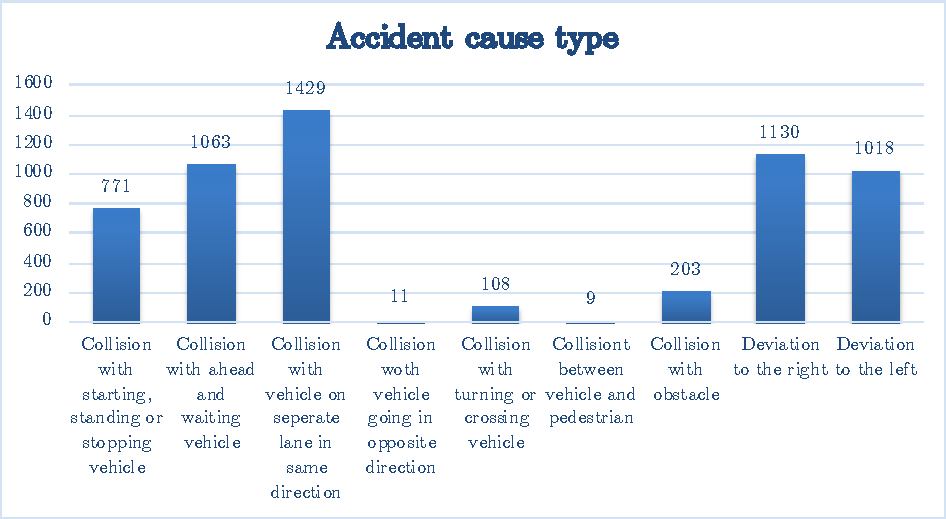
\includegraphics[scale=0.6]{./assets/baysis_dataset_UArt.pdf}
	\caption{Distribution of the accident cause type 'UArt'}
	\label{img:baysis_dataset_UArt}
\end{figure}

\paragraph{UArt}
The accident cause type, described by the two aggregated variables UArt1 and UArt2 (shown in figure \ref{img:baysis_dataset_UArt}), presents two major sets of causes. One being the accidents with waiting, stopping and starting vehicles in the same lane, which describe typical collision accidents during congested traffic. The other being the accidents in the next left or right lane, which describe common lane changing collisions. Accidents with cross traffic, pedestrians or opposite traffic are relatively uncommon. The variable does not show any order and is therefore of nominal type.

\begin{figure}[h]
	\centering
	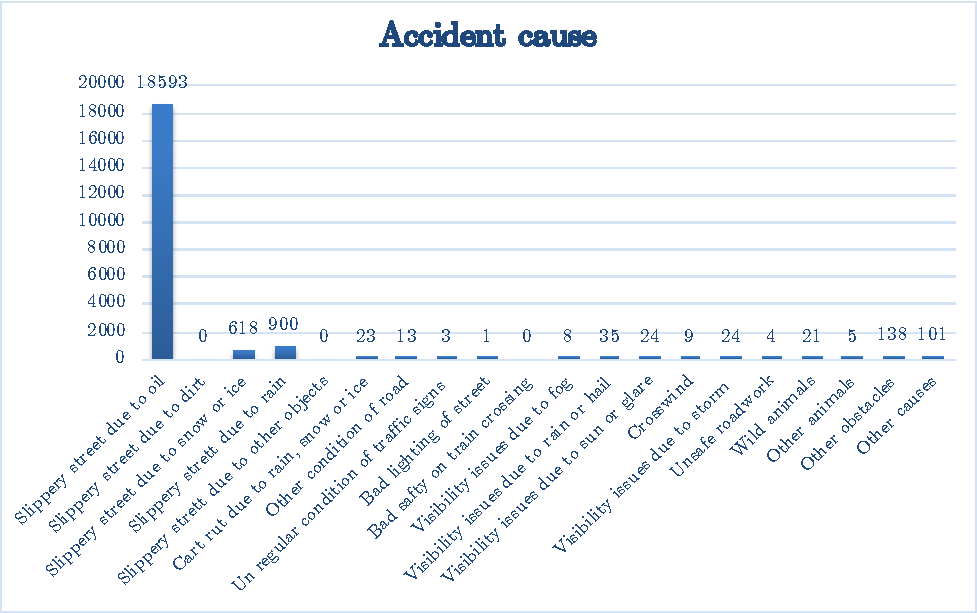
\includegraphics[scale=0.7]{./assets/baysis_dataset_AUrs.pdf}
	\caption{Distribution of the accident cause 'AUrs'}
	\label{img:baysis_dataset_AUrs}
\end{figure}

\paragraph{AUrs}
The summarized distribution of the parameters “AUrs1” and “AUrs2” (shown in figure \ref{img:baysis_dataset_AUrs}) does clearly that only the first category of “Slippery road condition due to oil” hold a significant share. Because of that any correlation to this parameter would not point to any usable statement and therefore can be neglected for the evaluation.

\begin{figure}[]
	\centering
	\includegraphics[scale=0.6]{./assets/baysis_dataset_Aufhi.pdf}
	\caption{Distribution of obstacle collision 'AufHi'}
	\label{img:baysis_dataset_Aufhi}
\end{figure}

\paragraph{AufHi}
The obstacle collision distribution (shown in figure \ref{img:baysis_dataset_Aufhi}) reveals that in most collision accidents car hit the guardrails. The other categories are rather uncommon. With 1,5\% of accidents without any collision, it can be stated that in most cases a collision is part of an accident. The counts of the remaining categories are insignificant. The variable does not show any order and is therefore of nominal type.

\begin{figure}[h]
	\centering
	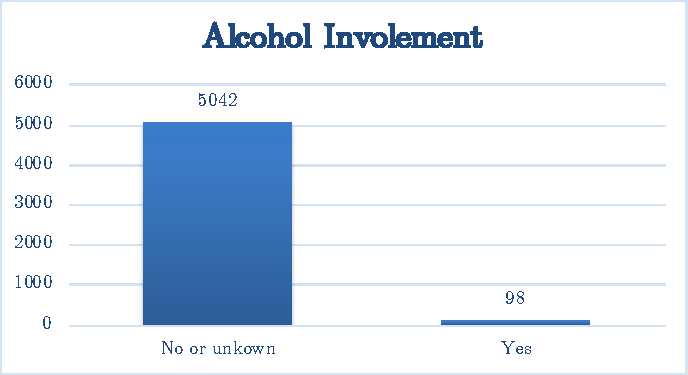
\includegraphics[scale=0.6]{./assets/baysis_dataset_Alkoh.pdf}
	\caption{Distribution of the alcohol Involvement 'Alkoh'}
	\label{img:baysis_dataset_Alkoh}
\end{figure}

\paragraph{Alkoh}
The Alcohol involvement indication parameter reveals that only 1,9\% of accidents have one or more involved persons with measurable blood alcohol. The variable only has two unique values and is therefore dichotomous.

\begin{figure}[h]
	\centering
	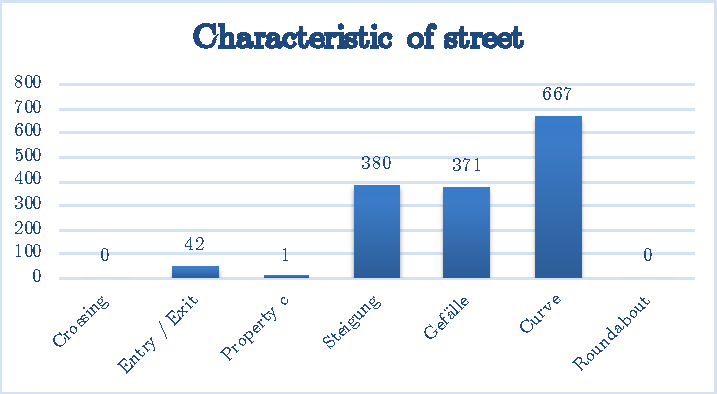
\includegraphics[scale=0.6]{./assets/baysis_dataset_Char.pdf}
	\caption{Distribution of the street characteristic 'Char'}
	\label{img:baysis_dataset_Char}
\end{figure}

\paragraph{Char}
The variable distribution shown in figure \ref{img:baysis_dataset_Char} describes the characteristic of the street where the accident happened. Since we are only considering highway, the type of "Crossing", "Property" and "Roundabout" is expected to be zero. The variabel is not ordered and therefore of nominal type.

\begin{figure}[h]
	\centering
	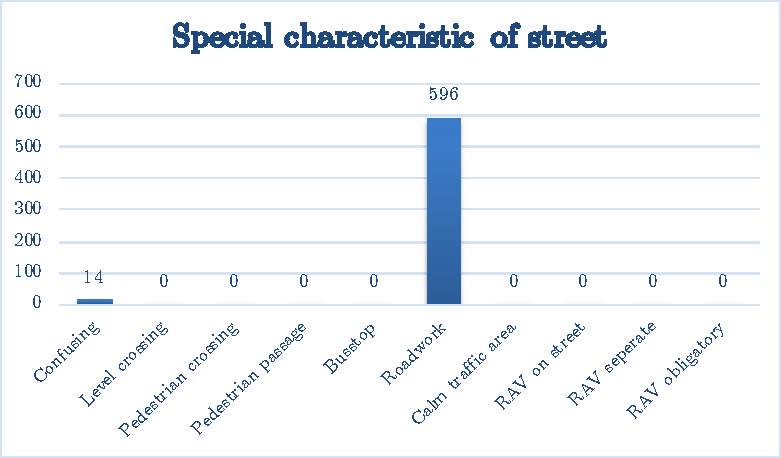
\includegraphics[scale=0.6]{./assets/baysis_dataset_Bes.pdf}
	\caption{Distribution of the special street characteristic 'Bes'}
	\label{img:baysis_dataset_Bes}
\end{figure}

\paragraph{Bes}
The aggregated distribution of the variables "Bes1", "Bes2" and "Bes3", which further defines the street characteristic mentioned above only has one significant share of the type "Roadwork". The variabel itself is therefore not suitable for a correlation analysis, but can be used as validation criterium for the matching of roadwork incidents.

\begin{figure}[h]
	\centering
	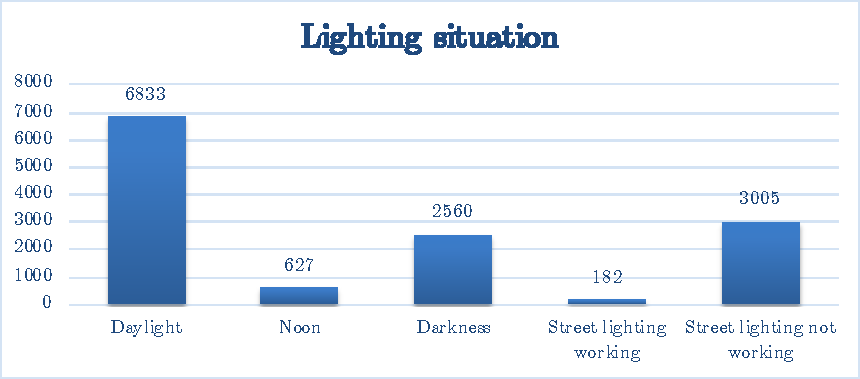
\includegraphics[scale=0.6]{./assets/baysis_dataset_Lich.pdf}
	\caption{Distribution of the lighting situation}
	\label{img:baysis_dataset_Lich}
\end{figure}

\paragraph{Lich}
The light situation parameter shown in \ref{img:baysis_dataset_Lich} does not reveal any features and describes the lighting condition when the accident happened. Because is could be ranked from best to works lighting is is of ordinal type.

\begin{figure}[h]
	\centering
	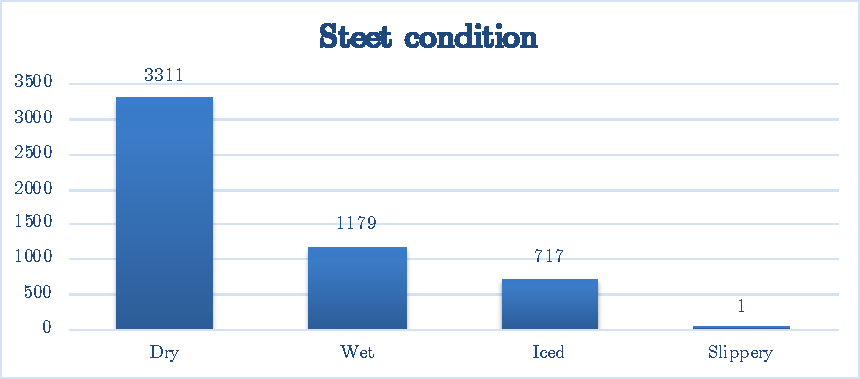
\includegraphics[scale=0.6]{./assets/baysis_dataset_Zust}
	\caption{Distribution of the street condition}
	\label{img:baysis_dataset_Zust}
\end{figure}

\paragraph{Zust}
Dolorem Ipsum. 

\begin{figure}[H]
	\centering
	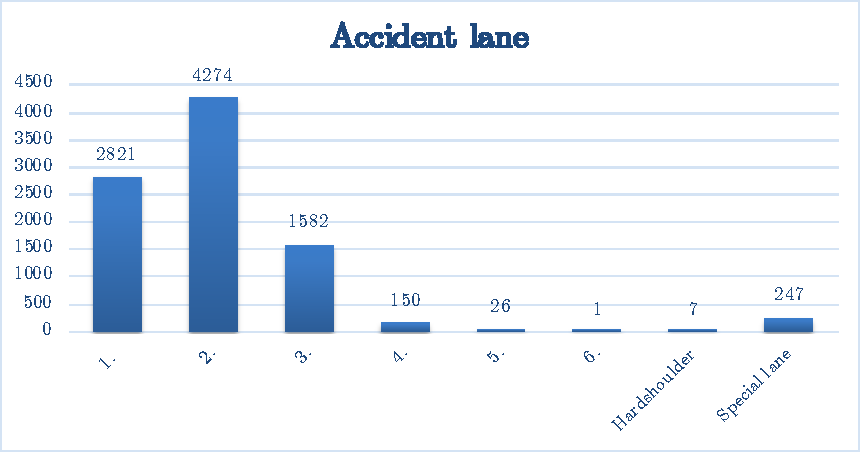
\includegraphics[scale=0.6]{./assets/baysis_dataset_Fstf.pdf}
	\caption{Distribution of accident lanes}
	\label{img:baysis_dataset_Fstf}
\end{figure}

\paragraph{Fstf}
sdfgsfg

\begin{figure}[H]
	\centering
	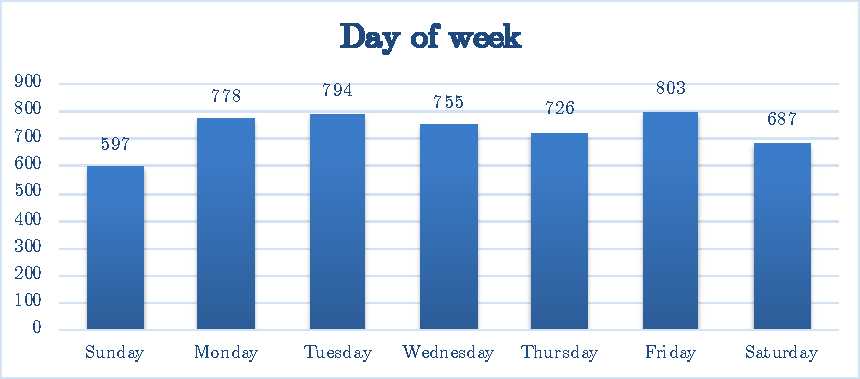
\includegraphics[scale=0.6]{./assets/baysis_dataset_WoTag.pdf}
	\caption{Distribution of week day}
	\label{img:baysis_dataset_Fstf}
\end{figure}

\paragraph{WoTag}
The variable of WoTag relates to the day of week, when the accident happened. 

\paragraph{FeiTag}
Form the total of 10262, 157 accidents took place on a public holiday. This is not a feature itself but the a possible correlation to jams could be that they are longer because of the increased traffic demand on holidays.

\bigskip

\bigskip

Table \ref{tab:table_baysis_paramters} show all categorized parameters, relevant for the correlation analysis, with variabel group, type and the format of the containing data.
	
\begin{table}[ht]
	\centering
	\begin{tabular}{c|c|c|c}
		\textbf{Variable} 	& \textbf{Group} 	& \textbf{Type} 		& \textbf{Format} \\
		\\[-1em]
		\hline
		\\[-1em]
		Kat  		& categorical 	& ordinal 	& numeric\\
		\\[-1em]
		\hline
		\\[-1em]
		Typ 		& categorical 	& nominal	& numeric\\
		\hline
		\\[-1em]
		Beteil 		& categorical 	& ordinal	& numeric\\
		\hline
		\\[-1em]
		UArt 		& categorical 	& nominal	& numeric\\
		\hline
		\\[-1em]
		AUrs 		& categorical 	& nominal	& numeric\\
		\hline
		\\[-1em]
		AufHi 		& categorical 	& nominal	& numeric\\
		\hline
		\\[-1em]
		Alkoh 		& categorical 	& dichotomous	& numeric\\
		\hline
		\\[-1em]
		Char 		& categorical 	& nominal	& numeric\\
		\hline
		\\[-1em]
		Bes 		& categorical 	& nominal	& numeric\\
		\hline
		\\[-1em]
		Lich 		& categorical 	& ordinal	& numeric\\
		\hline
		\\[-1em]
		Zust 		& categorical 	& ordinal	& numeric\\
		\hline
		\\[-1em]
		Fstf 		& categorical 	& nominal	& mixed\\
		\hline
		\\[-1em]
		WoTag 		& categorical 	& nominal	& text\\
		\hline
		\\[-1em]
		FeiTag 		& categorical 	& dichotomous	& numeric\\
	\end{tabular}
	\caption{Variable types of \acrshort{baysis} dataset}
	\label{tab:table_baysis_paramters}
\end{table}

To check for dependent variables which need to be considered in a correlation analysis, the correlation matrix for all relevant parameters in the BAYSIS dataset is calculated (see figures \ref{img:appendix_correlation_matrix_dataset_cramers} and \ref{img:appendix_correlation_matrix_dataset_theils}). Chramer's $V$ reveals several strong relationships, which are 'Typ'-'UArt1'. 'AUrs1'-'Zust1', 'AUrs1'-'Zust2' and some trivial relations of 'Char1'-'Char2', 'Bes1'-'Bes2', 'Lich1'-'Lich2'. That means that relations found in the later analysis, which contain the parameters 'Typ', 'UArt1, 'AUrs1, 'Zust1' and 'Zust2' might be in result of another depended variabel and should be checked for independence.

\bigskip

The designed evaluation tool, utilizes a PostgreSQL database for its data storage. Therefore the BAYSIS data in form of \acrfull{csv} needs to processed and converted into SQL data entities. Also, the data entities for each accident need to be uniform and comparable with our street network and other entities like roadworks, which makes it necessary to process and map the accidents onto our street network. After the necessary processing and import into the database, 7971 records end up being converted and persisted, which equivalent to 77,6\% of the total number of accidents. This 22,4\% of data loss is due to the conversion of from the BAYSIS geo-system to the HERE network, which tries to find a corresponding street network location to the legacy location of the BAYSIS dataset. If it is not able to locate the position of the BYSIS dataset on our street network, the record is discarded.

\section{ArbIS}
\label{dataset_arbis}

The \acrfull{arbis}, as described in chapter \ref{dataset_arbis}, is a collection service of all roadworks or maintenance planned, ongoing or finished on the Bavarian street network. With the 4500 long term and more than 40.000 short term building sites on German highways per year \cite{LAPID2018,Stmi2020}, road construction makes up for the majority of traffic obstructions in the summer months, when during the colder month, in which many kinds of construction projects are not possible, snow clearings or long-term constructions are the issue. That also means that the number and type of roadworks varies during the course of a year (StmB, 2020).

The dataset for 2019 contains close to 650.000 datapoints, which each describe the temporal and spatial extend, road name and number of closed lanes of a roadwork fragment. This fragmentation of events makes is rather hard to statically analyze this dataset since each roadwork is spitted into any number of fragments in now recognizable pattern and are only linked by a roadwork identifier. Therefore the analysis of the dataset in this section is rather basic. The import processing, similarly to the \acrshort{baysis} data in \ref{dataset_baysis}, and aggregation of fragments produces 282.839 roadwork events in the database. The monthly distribution of roadworks in the year 2019 is shown in figure \ref{img:arbis_dataset_monthly_absolute}.

\begin{figure}[h]
	\centering
	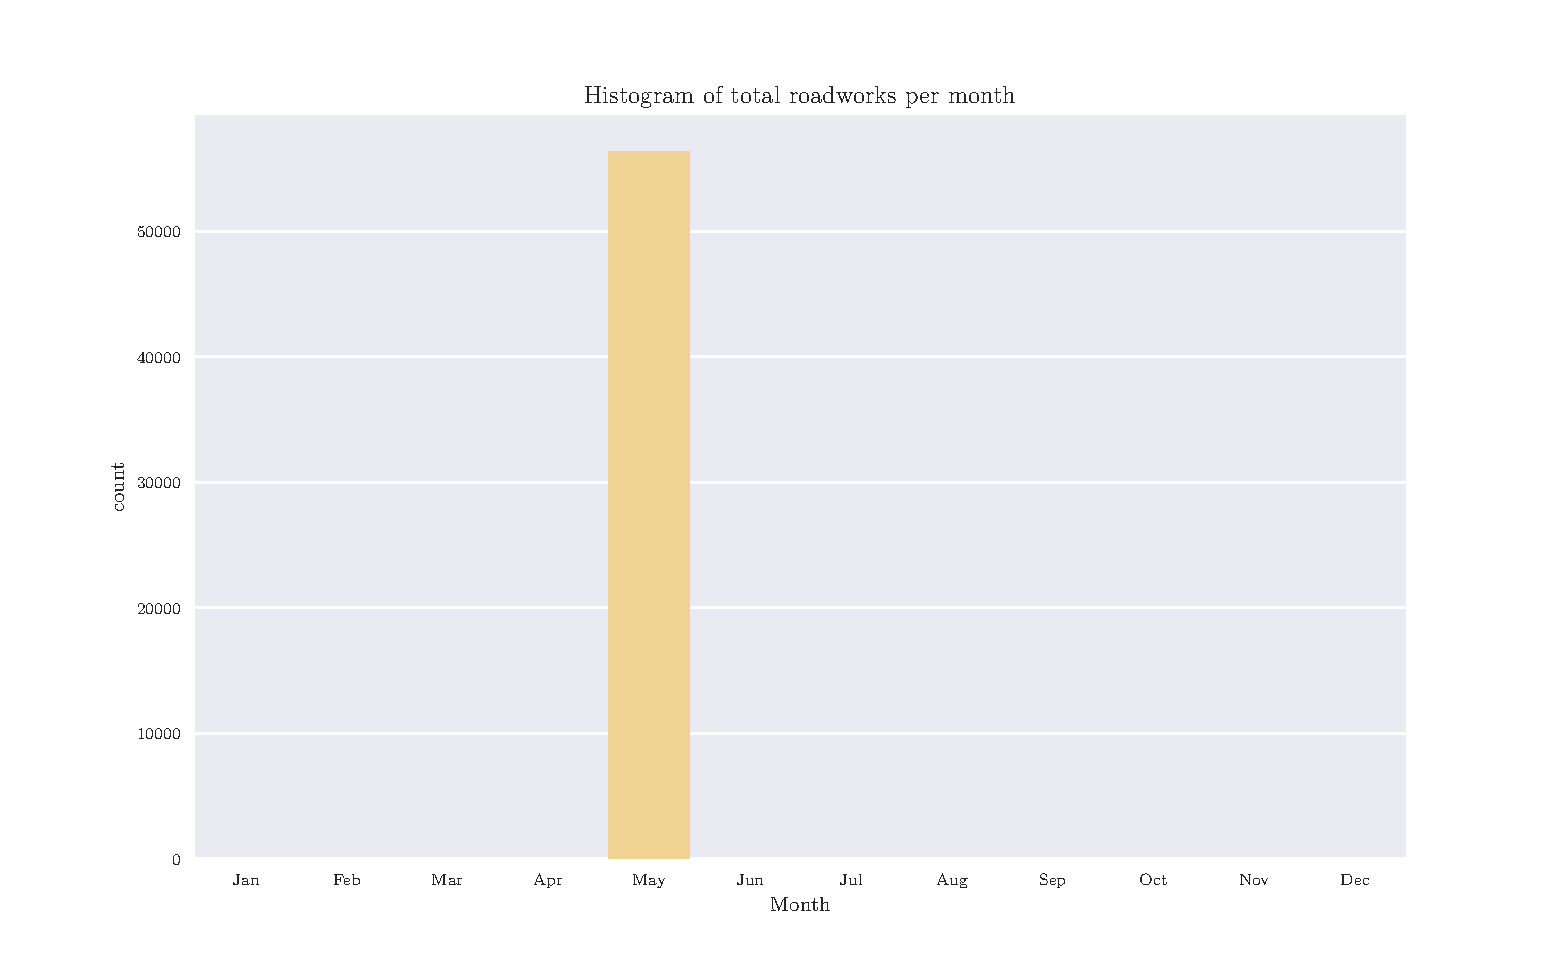
\includegraphics[width=0.7\textwidth]{../CorrAnalysis/data/ArbIS/01_dataset/plots/arbis_dataset_hist_month}
	\caption{Monthly distribution of absolute roadwork data entry counts}
	\label{img:arbis_dataset_monthly_absolute}
\end{figure}

The distribution shows that the winter months of January, February and December tend to have less roadwork that others, due to colder temperatures.

%\begin{figure}[h]
%	\centering
%	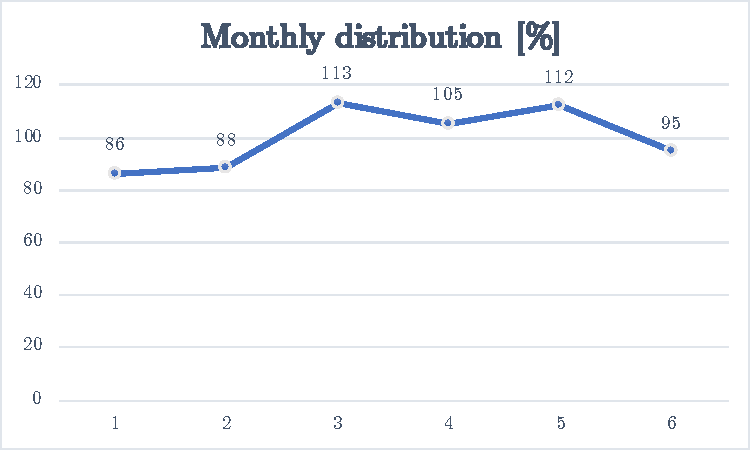
\includegraphics[width=0.7\textwidth]{./assets/arbis_dataset_monthly_percentage.pdf}
%	\caption{Monthly distributions of roadwork data entry counts in percentages to mean}
%	\label{img:arbis_dataset_monthly_percentage}
%\end{figure}

\subsubsection{Strasse}



%\begin{tabular}{lrrrrrrr}
\toprule
{} &  Strasse &  AnzGesperrtFs &  Einzug &  Richtung &  Month &  Length &  Duration \\
\midrule
Strasse       &      NaN &         0.0000 &  0.0000 &    0.0000 &    0.0 &  0.0000 &    0.0000 \\
AnzGesperrtFs &      0.0 &            NaN &  0.0000 &    0.2547 &    0.0 &  0.0000 &    0.0000 \\
Einzug        &      0.0 &         0.0000 &     NaN &    0.0000 &    0.0 &  0.0006 &    0.0000 \\
Richtung      &      0.0 &         0.2547 &  0.0000 &       NaN &    0.0 &  0.0000 &    0.0489 \\
Month         &      0.0 &         0.0000 &  0.0000 &    0.0000 &    NaN &  0.0000 &    0.0000 \\
Length        &      0.0 &         0.0000 &  0.0006 &    0.0000 &    0.0 &     NaN &    0.0000 \\
Duration      &      0.0 &         0.0000 &  0.0000 &    0.0489 &    0.0 &  0.0000 &       NaN \\
\bottomrule
\end{tabular}


\chapter{Methodology}
\label{methodology}
The previous chapters gave an introduction into the systems, data and statistical indicators which will be used to determine if jams characteristics, detected in \acrshort{fcd} and incident characteristics from accidents (\acrshort{baysis}) and roadworks (\acrshort{arbis}) are statistically dependent on each other. The research question to be answered stands as follows:

\begin{center}
	\textit{Do congestion- and incident-characteristics correlate?}
\end{center}

\medskip

The methodology to answer these research questions, will be elaborated in this chapter, starting with the detection of jams in the FCD. This also contains the generation of congestion characteristics and collection of adjacent incident. The \acrshort{fcd} is a continuous time series of datapoint which represents the mean absolute and relative speed of the street section at each 3-minute interval on a road section. In \ref{dataset_fcd} we determined that thought a manual visual analysis jams can be easily identified. This manual identification will be automated because of the amount of data representing a complete year and all Bavarian highways. The gathered tuples of congestion and incident are then processed and exported into a unified data-structure. 

The \gls{evaltool} from the \gls{congstats} service, the project which inspired this thesis, was developed for this purpose and will be expanded with required features. Afterward the stored dataset of congestion and incidents events will be analyzed for correlations and other statistic indicators.

\bigskip

\section{Detection Algorithm}
First step is the detection of congestion events. The definition in \ref{definition_congestion} states that a congestion is a dense, timely and spatial accumulation of jammed cells, also describable as cluster of jammed cells. Therefore a clustering algorithm would be suitable to identify congestion events.

For the classification of the congestion events into different types, by theirs spatial and timely extends a shaping algorithm is needed. It is supposed to convert the accumulation of cells into a simple describable shape, which can be put into groups.

\subsection{Clustering}
\label{methodology_clustering}
The term clustering is the short form of a data mining technique also called numerical taxonomy or cluster analysis with the goal of finding data structures or associations. For this purpose a multitude of algorithms where developed over time, varying in they strategies, methods and performance \cite{Busch2004}. For example k-means or k-metoid (point distance), affinity propagation (graph distance), mean-shift (point distance), DBSCAN (nearest point distance), gaussian mixtures (mahalanobis distance to centers) or spectral clustering (graph distance), which can be sorted into the categories of partition-based, hierarchical-based and density-based clustering \cite{Chauhan2020,Yildirim2020}.

% https://texample.net/tikz/examples/probability-tree/
% https://webis.de/downloads/theses/papers/busch_2005.pdf 1.6
%\begin{tikzpicture}[grow=right, sloped]
%\node[bag] {Cluster Algorithms}
%    child {
%        node[bag] {hierarchic}        
%             child {
%                node[end, label=right:
%                    {single-linkage, group-average}] {}                
%                edge from parent
%            }         
%            edge from parent 
%    }
%    child {
%        node[bag] {iterative}        
%            child {
%                node[end, label=right:
%                    {k-means, k-metoid, Kerninghan-Lin}] {}                
%                edge from parent
%            }         
%            edge from parent 
%    }
%    child {
%        node[bag] {density-based}        
%            child {
%                node[end, label=right:
%                    {DBSCAN, MajorClust}] {}                
%             	edge from parent
%            }
%            edge from parent
%    }
%	child {
%        node[bag] {meta-search}        
%                 child {
%                node[end, label=right:
%                    {genetic algorithms}] {}
%                edge from parent
%            }            
%            edge from parent
%    }
%    child {
%        node[bag] {statistical}        
%        child {
%                node[end, label=right:
%                    {gaussian mixtures}] {}
%                edge from parent
%            }
%            edge from parent         
%    };
%\end{tikzpicture}

\bigskip

\begin{figure}[h]
	\centering
	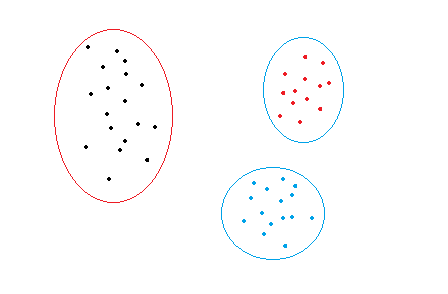
\includegraphics[scale=0.5]{./assets/cluster_seperate.png}
	\caption{Example clustered by k-means algorithm \cite{Yildirim2020}}
	\label{cluster_kmeans}
\end{figure}

To illustrate which problems can occur when using cluster algorithms and to defined the features which makes algorithm suitable, the k-means is used as base comparison. The figure \ref{cluster_kmeans} shows three differently colored groups of points, which are clustered into three clusters, represented by the circles around the groups. It demonstrates the general principle of clustering and was done by the common k-means algorithm with the $a$ $priori$ parameter of three clusters. 

\begin{figure}[h]
	\centering
	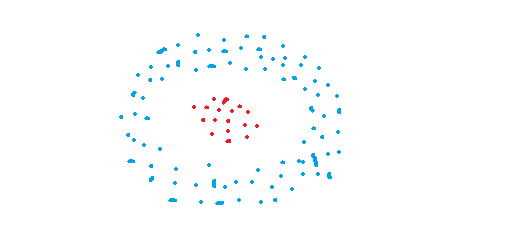
\includegraphics[scale=0.4]{./assets/cluster_1.png}
	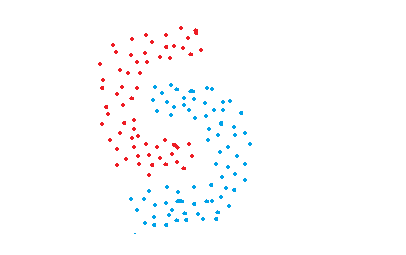
\includegraphics[scale=0.4]{./assets/cluster_2.png}
	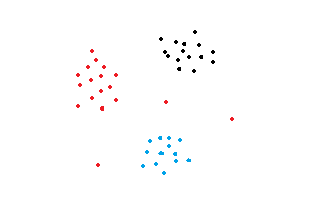
\includegraphics[scale=0.4]{./assets/cluster_3.png}
	\caption{Example clustered by density-based algorithm \cite{Yildirim2020}}
	\label{cluster_dbscan}
\end{figure}

This works well as long as the groups don't overlay, intersect or have arbitrary shapes like in the figures \ref{cluster_dbscan}. When this is the case, the k-mean may cluster loosely related point together, which actually are more strongly related to other points, because it considers every point as possible neighbor. Since jams in FCD data can overlay and have any number of shape, as suitable algorithms need to be able to handle such data.

Another issue with many clustering alorithms is the increasing runtime when processing larger amounts of data. The objective function \ref{formula_kmeans} of the examplatory k-mean states that $n$ distances are calculated for $k$ points \cite{Santhanam2010}. With the assumption that every distance for every point will be calculated and therefore $k=n$, the Big $\Theta$ notation, commonly known as Big $O$, describing the scaleable time complexity of an algorithm, is $O(n \cdot K \cdot I \cdot d)$ ($n$ = number of points, $K$ = number of clusters, $I$ = number of iterations, $d$ = number of attributes) \cite{Dalatu2016}. It is commonly simplified in literature to $O(n^2)$, a quadratic complexity \cite{Pakhira2014}. The assumption also entails that in a worst case scenario $n^2$ calculations have to be computed over all iterations.

\begin{equation}
\label{formula_kmeans}
	k_{mean} =  \sum_{j=1}^k{\sum_{i=1}^n{\abs{x_i^j-c_j}}}
\end{equation}

\bigskip

A Big $O$ notation of $O(n^2)$ can generally be described as inefficient, but if we would apply the worst case scenario as an example on the data of the highway A3 and a timeframe of 24 hours, which contains 836.752 data points, the runtime issue becomes quite obvious. As the equation \ref{equation_kmeans_nn} show, the total number of calculation is so quite high, resulting in a considerable runtime. \cite{Busch2004}

\begin{equation}
\label{equation_kmeans_nn}
	 = 836752 \cdot 836752 = 700.153.909.504 = 7 \cdot 10^{11}
\end{equation}

\bigskip

Entering density-based methods, which are better suited to identify distinctive, arbitrary clusters in, by looking for a contiguous region of high point density, separated from others by contiguous regions of low point density \cite{Chauhan2020}. These do not necessarily have less runtime, but better cluster representation.

\subsubsection{Algorithm}

The DBSCAN algorithm, standing for \textbf{d}ensity-\textbf{b}ased \textbf{s}patial \textbf{c}lustering of \textbf{a}pplications with \textbf{n}oise, is able to find arbitrary shaped cluster and clusters by considering the spatial density, which also represents noise. The basic idea of this algorithm is to form cluster of points, which are close too \textbf{many} other points of the cluster. For this strategy two thresholds parameters are needed. The first being the minimal size of a cluster, referred to as $MinPts$, which defines the minimum number of points necessary to form a cluster. And secondly the maximum distance threshold between points, $eps$ ($\varepsilon$), to be considered as neighbors and become part of a cluster. These thresholds classify a data point as core point, (directly) density-reachable point or noise. \cite{Yildirim2020,Chauhan2020,Padro2017}

\begin{itemize}
	\item A \textbf{core} point $q$ has at least $MinPts$ points around them within the neighborhood $\varepsilon$, including itself.
    \item \textbf{Directly density-reachable} border points have at least one core point within the neighborhood $\varepsilon$.
     \item \textbf{Density-reachable} border points have at least one core point within the neighborhood $\varepsilon$ of a cain of points $p_1,p_2,...p_n$.
 	\item \textbf{Noise} or outliner point are neither core points nor are they density-reachable and therefore have less than $MinPts$ in their neighborhood $\varepsilon$, including itself.
\end{itemize}

The general procedure of the algorithm is as follows \cite{Zhao2018}, with the input of $n$ points, neighborhood radius $\varepsilon$ and density threshold $MinPts$:

\begin{itemize}
	\item[\textbf{1.}] Mark all points as \textit{unvisited}
	\item[\textbf{2.}] Choose point $p$ randomly from all \textit{unvisited} points.
	\begin{itemize}
		\item[\textbf{a.}] Choose point $p$ randomly from all \textit{unvisited} points and mark $p$ as \textit{visited}.
		\item[\textbf{b.}] Count points in the neighborhood $\varepsilon$ to check if $p$ is core point. If $p$ is core point, create new cluster $C$ and add all directly density-reachable and \textit{unvisited} points. Otherwise mark $p$ as noise.
		\item[\textbf{c.}] Choose point $p'$ randomly from all \textit{unvisited} points of $C$ and mark $p$ as \textit{visited}.
		\item[\textbf{d.}] Count points in the neighborhood $\varepsilon$ to check if $p'$ is core point. If $p$ is core point add all directly density-reachable points, which do not already belong to a cluster, to $C$. Otherwise mark $p$ as noise.
		\item[\textbf{e.}] Repeat \textbf{c} and \textbf{d} until there are no \textit{unvisited} points left in $C$.	
	\end{itemize} 
	\item[\textbf{3.}] Repeat \textbf{2} until all points are \textit{visited} 
\end{itemize}

%https://www.kde.cs.uni-kassel.de/wp-content/uploads/ws/LLWA03/fgml/final/Kirchner.pdf
%https://www.researchgate.net/publication/322729622_Characterizing_Diffusion_Dynamics_of_Disease_Clustering_A_Modified_Space-Time_DBSCAN_MST-DBSCAN_Algorithm
%https://www.nature.com/articles/s41598-017-12852-z
%http://citeseerx.ist.psu.edu/viewdoc/download?doi=10.1.1.63.1629&rep=rep1&type=pdf
%http://cucis.eecs.northwestern.edu/publications/pdf/HAL18.pdf

\subsubsection{Distance Measuring}
The algorithm is based on the density of points. This density representation is achieved via checking the neighborhood $\varepsilon$ against calculation of distance from point $A$ to $B$, typical the Euclidean distance, which is based on the pythagorean theorem (see equation \ref{formula_euclidean} \cite{Erhard2020}).

\begin{figure}[h]
	\centering
	
	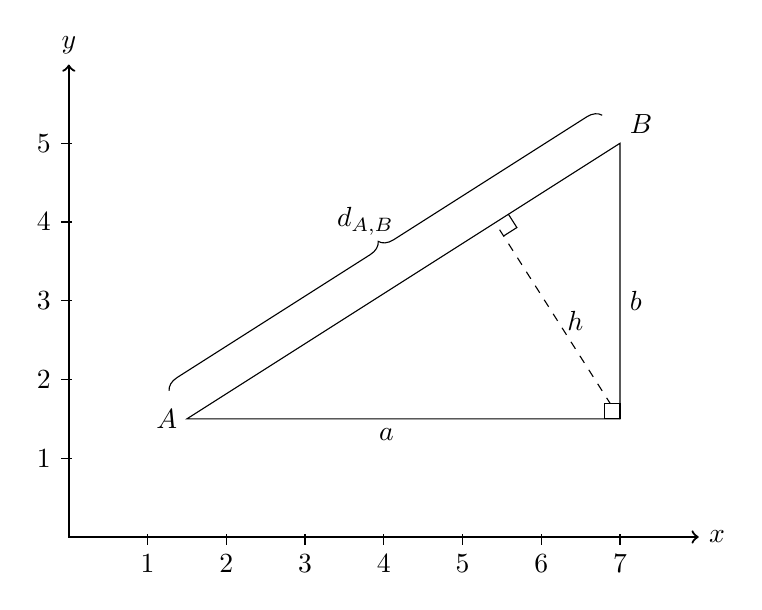
\begin{tikzpicture}[scale=1.0]
	
	\draw [<->,thick] (0,6) node (yaxis) [above] {$y$}
        |- (8,0) node (xaxis) [right] {$x$};
        
    \foreach \x in {1,...,7}
    	\draw (\x,1pt) -- (\x,-3pt)
		node[anchor=north] {\x};
		
	\foreach \y in {1,...,5}
    	\draw (1pt,\y) -- (-3pt,\y) 
     	node[anchor=east] {\y}; 

	\coordinate[label={270:$$}] (C) at (7,1.5);
	\coordinate[label={180:$A$}] (A) at (1.5,1.5);
	\coordinate[label={30:$B$}] (B) at (7,5);

	\draw (C) -- (A)node[midway,below left]{$a$} -- (B)  -- cycle node[midway,below right]{$b$};
       
	\draw [dashed] (C) -- ($(A)!(C)!(B)$) coordinate (P) node [midway, right]{$h$};
	
	\draw[decorate,decoration={brace,raise=12pt,amplitude=5pt}] (A) -- (B);
	
	\path (B) -- (P) node[midway,above]{$$}-- (A) node[midway,above]{$$} ($($(A)!0.5!(B)$)!0.9cm!90:(B)$) node {$d_{A,B}$}; % You can nest calc syntax!
	
	\filldraw[fill=white] (C) -- ($(C)!2mm!(A)$) coordinate (U) -- ($(U)!2mm!90:(C)$) 
      --($(C)!2mm!(B)$) --cycle;
	
	\draw ($(P)!2mm!(C)$) coordinate (V) -- ($(V)!2mm!90:(C)$) --($(P)!2mm!(B)$);

	\end{tikzpicture}
\end{figure}

\medskip

\begin{equation}
	d_{A,B} = \sqrt{a^2 + b^2} = \sqrt{(x_B-x_A)^2+(y_B-y_A)^2}
	\label{formula_euclidean}
\end{equation}

\medskip

As shown above, the euclidean distance calculation assumes a Euclidean spaces, meaning equal scaling of both axis, which is not the case with FCD. The space of the FCD is defined by a spatial and a temporal dimension, which are scaled differently as mentioned in section \ref{dataset_fcd}. This 2-dimensional space can be visualized like:

TODO figure of FCD, non euclidean space 



The threshold for the virtual travel time gap in-between congestion events during the cluster consolidation. 

\begin{itemize}
	\item Spatial gap : $l_{min,gap} = 5000$ % cluster consolidation 
	\item Temporal gap : $t_{min,gap} = 6 min$ % cluster consolidation 
	\item Virtual travel-time gap $t_{min,gap}^{virtual} = 360s$
\end{itemize}
% TODO read and add infos
% https://diglib.tugraz.at/download.php?id=576a764ebc982&location=browse \cite{Hatbauer2011}

\subsubsection{Calibration}

%Parameter estimation:
%The parameter estimation is a problem for every data mining task. To choose good parameters we need to understand how they are used and have at least a basic previous knowledge about the data set that will be used.
%eps: if the eps value chosen is too small, a large part of the data will not be clustered. It will be considered outliers because don’t satisfy the number of points to create a dense region. On the other hand, if the value that was chosen is too high, clusters will merge and the majority of objects will be in the same cluster. The eps should be chosen based on the distance of the dataset (we can use a k-distance graph to find it), but in general small eps values are preferable.
%minPoints: As a general rule, a minimum minPoints can be derived from a number of dimensions (D) in the data set, as minPoints ≥ D + 1. Larger values are usually better for data sets with noise and will form more significant clusters. The minimum value for the minPoints must be 3, but the larger the data set, the larger the minPoints value that should be chosen.
%\cite{Padro2017}

\subsubsection{Performance Tuning}
Leaving out the runtime implication pf the distnace mesaurer the DBSCAN 
%The complexity of DBSCAN Clustering Algorithm
% 
%
%Best Case: If an indexing system is used to store the dataset such that neighborhood queries are executed in logarithmic time, we get O(nlogn) average runtime complexity.
%Worst Case: Without the use of index structure or on degenerated data (e.g. all points within a distance less than ε), the worst-case run time complexity remains O(n²).
%Average Case: Same as best/worst case depending on data and implementation of the algorithm.
%\cite{Chauhan2020}

\subsection{Shaping}
\label{methodology_shaping}

Convex Hull
%https://www.diva-portal.org/smash/get/diva2:931027/FULLTEXT02
\begin{figure}[h]
	\centering
	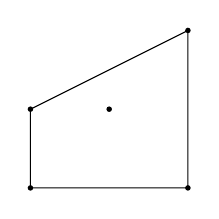
\begin{tikzpicture}
  	% doesn't work:
  	%\draw[mark=*] convex hull[points={(0,0),(1,1),(2,2),(0,1),(2,0)}];
     	
  	%should produce something similar to the following:
  	\draw (0,0) -- (0,1) -- (2,2) -- (2,0) -- cycle;
  	\foreach \point in {(0,0),(1,1),(2,2),(0,1),(2,0)} {
    	\fill[black] \point circle[radius=1pt];
  	}
	\end{tikzpicture}
\end{figure}


\section{Matching Algorithm}
\label{methodology_matching}
We now have a list of jams, found on the matching incidents with spatial and timely adjacent congestions
See CONGSTATS Matching Algorithm (own implementation)

\section{Data Processing}
\label{methodology_data_processing}
Until now all data is in the CONGSTATS system. Export to analyzable format is necessary.
Which values where converted into numeric values and why and …

% TODO read and use a source for loss parameter
% file:///Users/jakoberpf/Downloads/neuberechnung-der-stauzeitkosten%20.pdf
%\begin{itemize}
%	\item The cost rate for one car loosing one hour travel time [€/(Fz*h)] cost.rate.car=11
%	\item The cost rate for one truck / heavy goods vehicle loosing one hour travel time [€/(Fz*h)] cost.rate.hgv=25
%\end{itemize}

The congestion object is expanded with...

The temporal reference of if the incident to the congestion (\textbf{temporalGlobalLoc}). The incident...
\begin{itemize}
	\setlength\itemsep{0em}
	\item[1] = is before
	\item[2] = is after
	\item[3] = is during
	\item[4] = is overlapping before
	\item[5] = is overlapping after
\end{itemize}

The spatial reference of if the incident to the congestion (\textbf{spatialGlobalLoc}). The incident...
\begin{itemize}
	\setlength\itemsep{0em}
	\item[0] = is before or after
	\item[1] = is during
\end{itemize}

The temporal reference of if the incident is during the congestion (\textbf{temporalInternalLoc}). The incident is within...
\begin{itemize}
	\setlength\itemsep{0em}
	\item[1] = 10\,\% to Beginning
	\item[2] = 10\,\% - 30\,\% to Beginning
	\item[3] = 30\,\% - 70\,\% (Middle)
	\item[4] = 30\,\% - 10\,\% to Ending
	\item[5] = 10\,\% to Ending
\end{itemize}

The spatial reference of if the incident is during the congestion (\textbf{spatialInternalLoc}). The incident is within...
\begin{itemize}
	\setlength\itemsep{0em}
	\item[1] = 10\,\% to Beginning
	\item[2] = 10\,\% - 30\,\% to Beginning
	\item[3] = 30\,\% - 70\,\% (Middle)
	\item[4] = 30\,\% - 10\,\% to Ending
	\item[5] = 10\,\% to Ending
\end{itemize}
    
    
\section{Correlation Processing}
\label{definition_correlation_processing}

Explain python script for correlation analysis, based on \cite{Potvin2020}

\chapter{Analysis}

Analysis of the resulting separate datasets of congestion and incidents. What characteristic and key indicators are prominent?
\section{Features}
What find of values, features and so on, does the dataset contain?
\section{Time and space dimension}
What time frame does the dataset cover and over what spatial area.
\section{Containing information}
What kind of information does the dataset contain?
\section{Integrity and short comings}
What kind of information does the dataset contain?

\chapter{Interpretation}

\section{Assocations}

\section{Predictions}
Is the correlation strong enough to use it for predicting congestions and accidents?

\subsection{Prediction of Accidents}

\subsection{Prediction of Congestions}

\chapter{Implementation}

\section{Requirements}

\section{Data Aviability}

\chapter{Conclusion}

\section{Answer of research question}

\section{Usability of results and interpretation}

\section{Future development and possible improvements} 

\subsubsection{intraclass correlation coefficient (ICC)}
Usage of ICC instead of Eta and Kruskal-Wallis H.
% https://stats.stackexchange.com/questions/73065/correlation-coefficient-between-a-non-dichotomous-nominal-variable-and-a-numer
% https://pingouin-stats.org/generated/pingouin.intraclass_corr.html

\subsubsection{Improve DBSCAN}
The improved DBSCAN algorithm based on cell-like P systems with promoters and inhibitors
% https://journals.plos.org/plosone/article?id=10.1371/journal.pone.0200751

\subsubsection{Clustering in 3D (including cell speed)}
Expand DBSCAN to three dimension from space and time (2D) to include cell speed into clustering algorithm.

%\subsubsection{... Test}
%\paragraph{... Test}
%\subparagraph{... Test}

\addcontentsline{toc}{chapter}{Bibliography}
\bibliographystyle{apalike}
\bibliography{../Literatur/library}{}

\addcontentsline{toc}{chapter}{List of Figures}
\listoffigures

\addcontentsline{toc}{chapter}{List of Tables}
\listoftables

\printglossary[title=List of Acronyms, type=\acronymtype]

\printglossary[title=List of Terms]

\begin{appendices}

\chapter{BAYSIS Dataset Figures}
\label{appendix_baysis}

%\tocless\section{}
\newgeometry{left=1cm,right=1cm,top=1cm,bottom=2cm}
\begin{figure}[h]
	\centering
	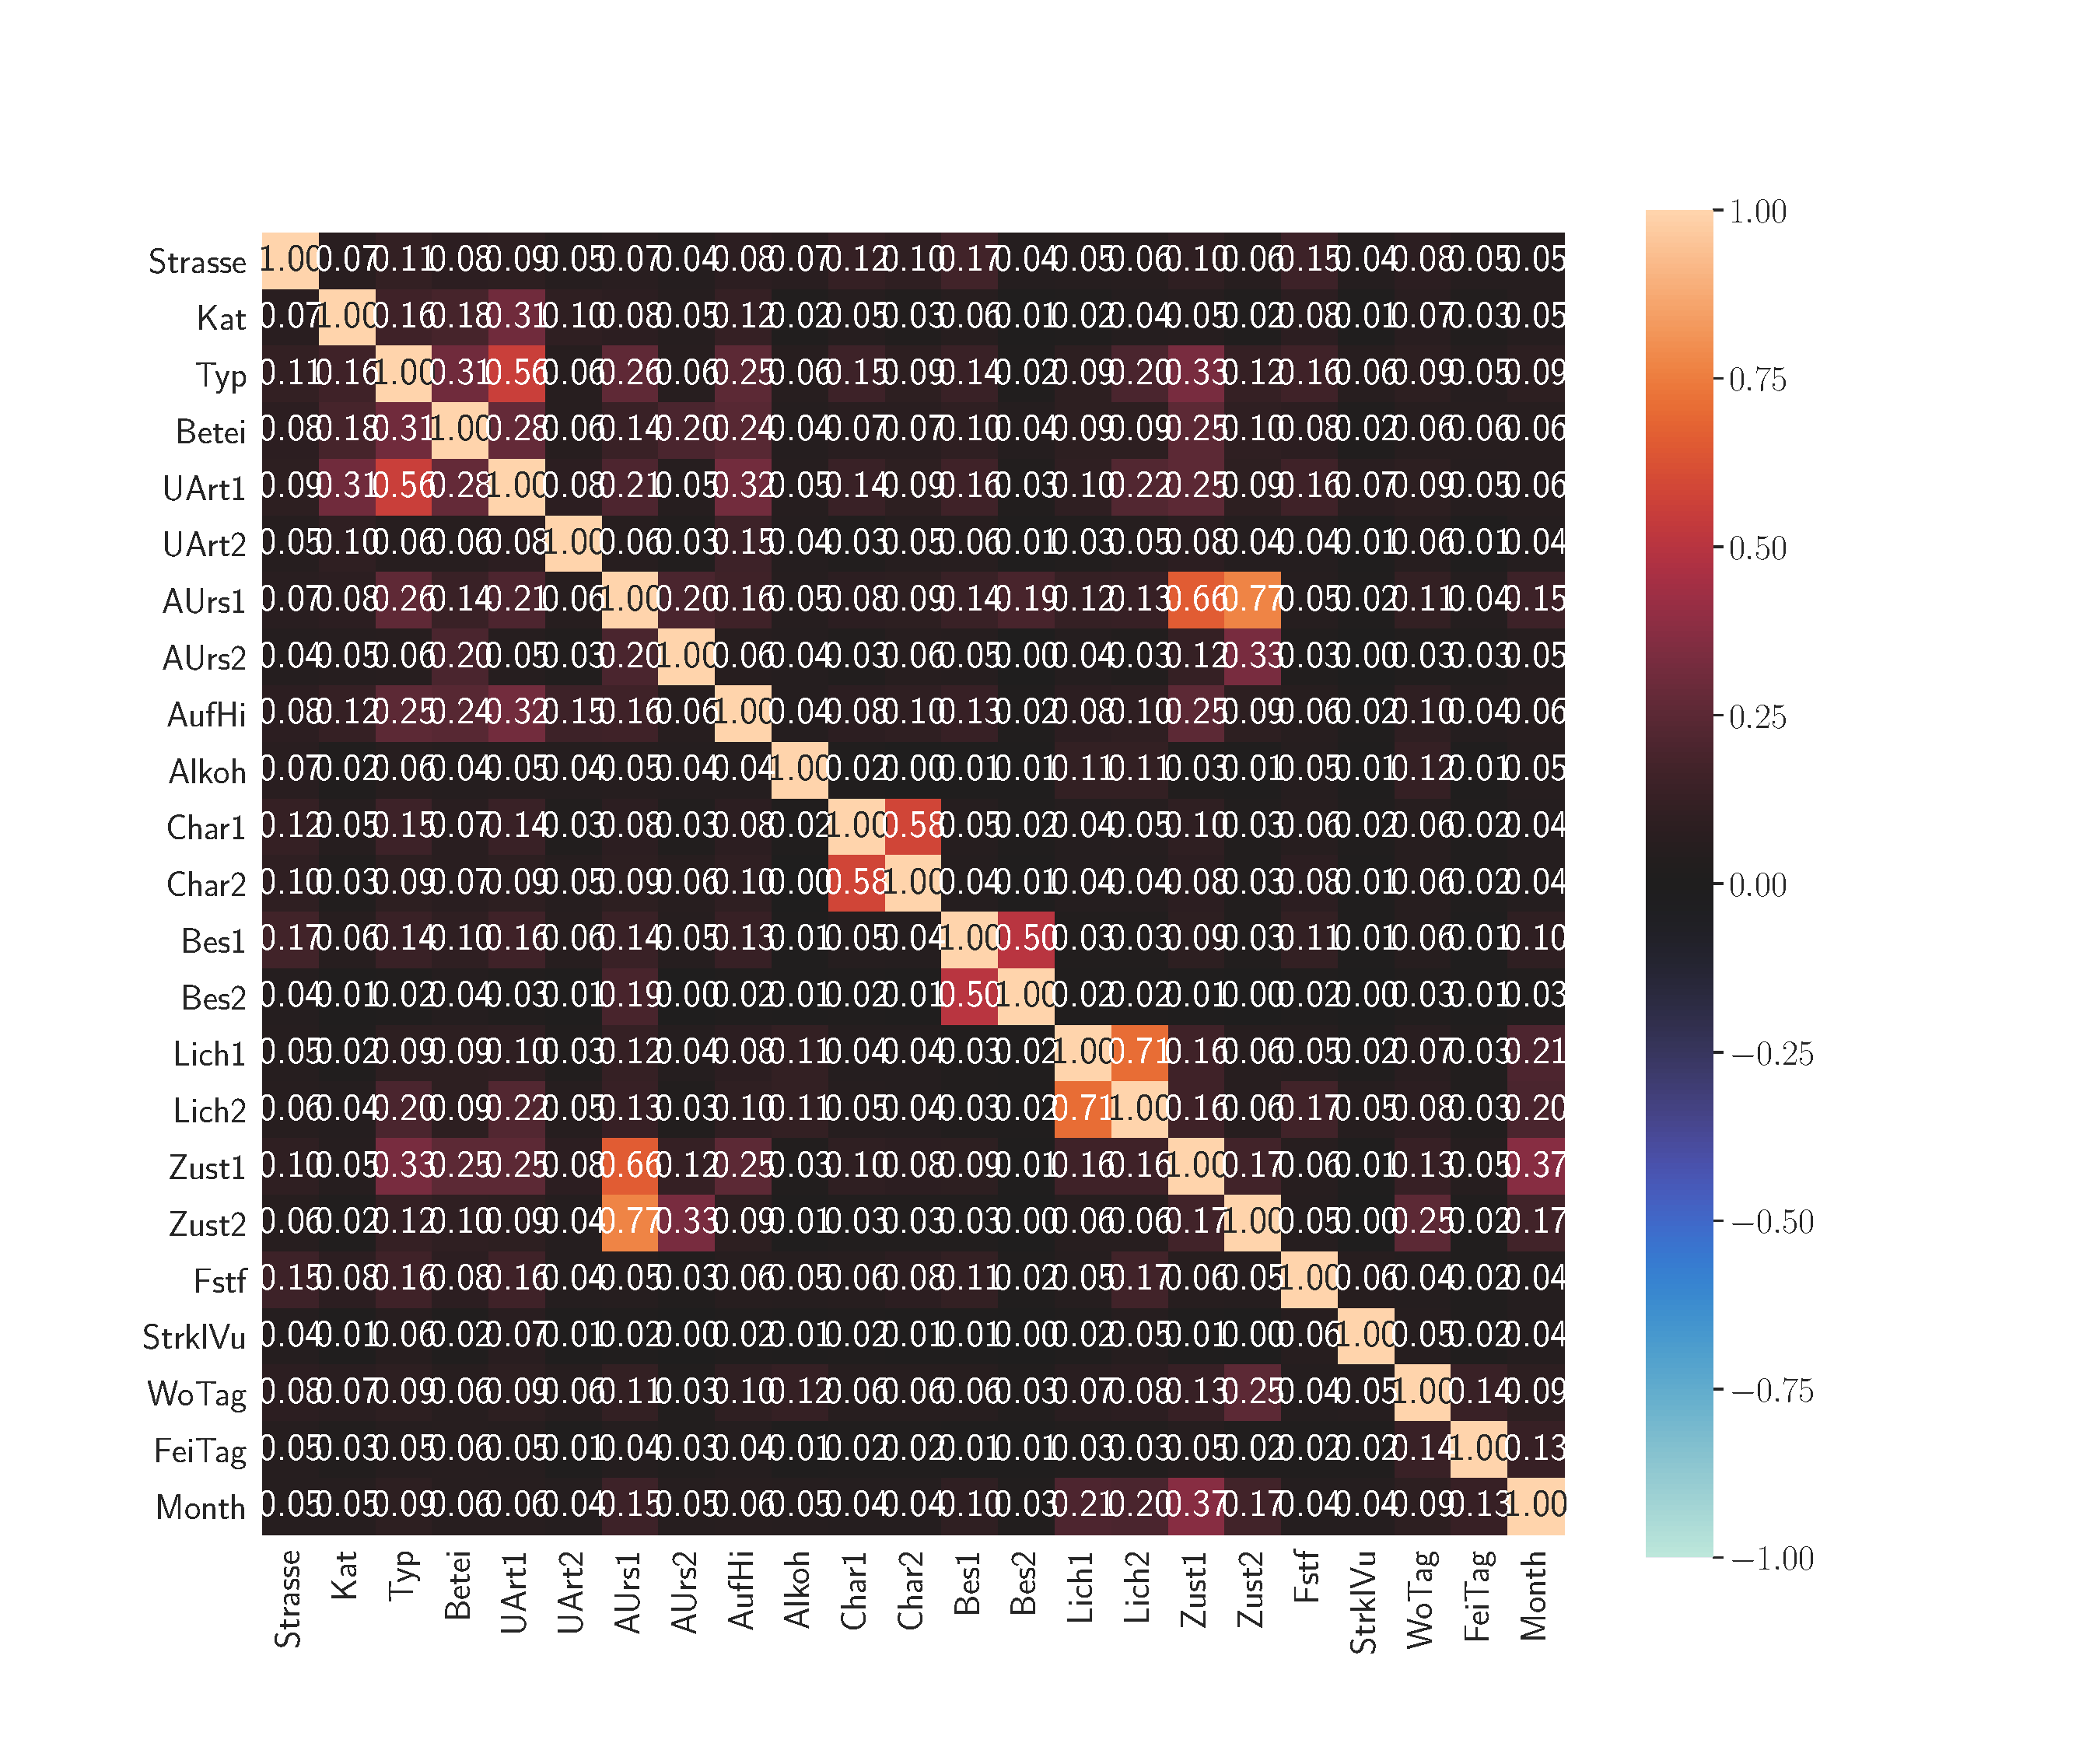
\includegraphics[scale=0.4]{../CorrAnalysis/data/BAYSIS/01_dataset/plots/baysis_dataset_corr_cramers}
	\caption{Correlation matrix for BAYSIS dataset, with Cramer's $V$}
	\label{img:appendix_correlation_matrix_dataset_cramers}
\end{figure}
\restoregeometry

%\tocless\section{}
\newgeometry{left=1cm,right=1cm,top=1cm,bottom=2cm}
\label{appendix_baysis_dataset_corr_theils}
\begin{figure}[h]
	\centering
	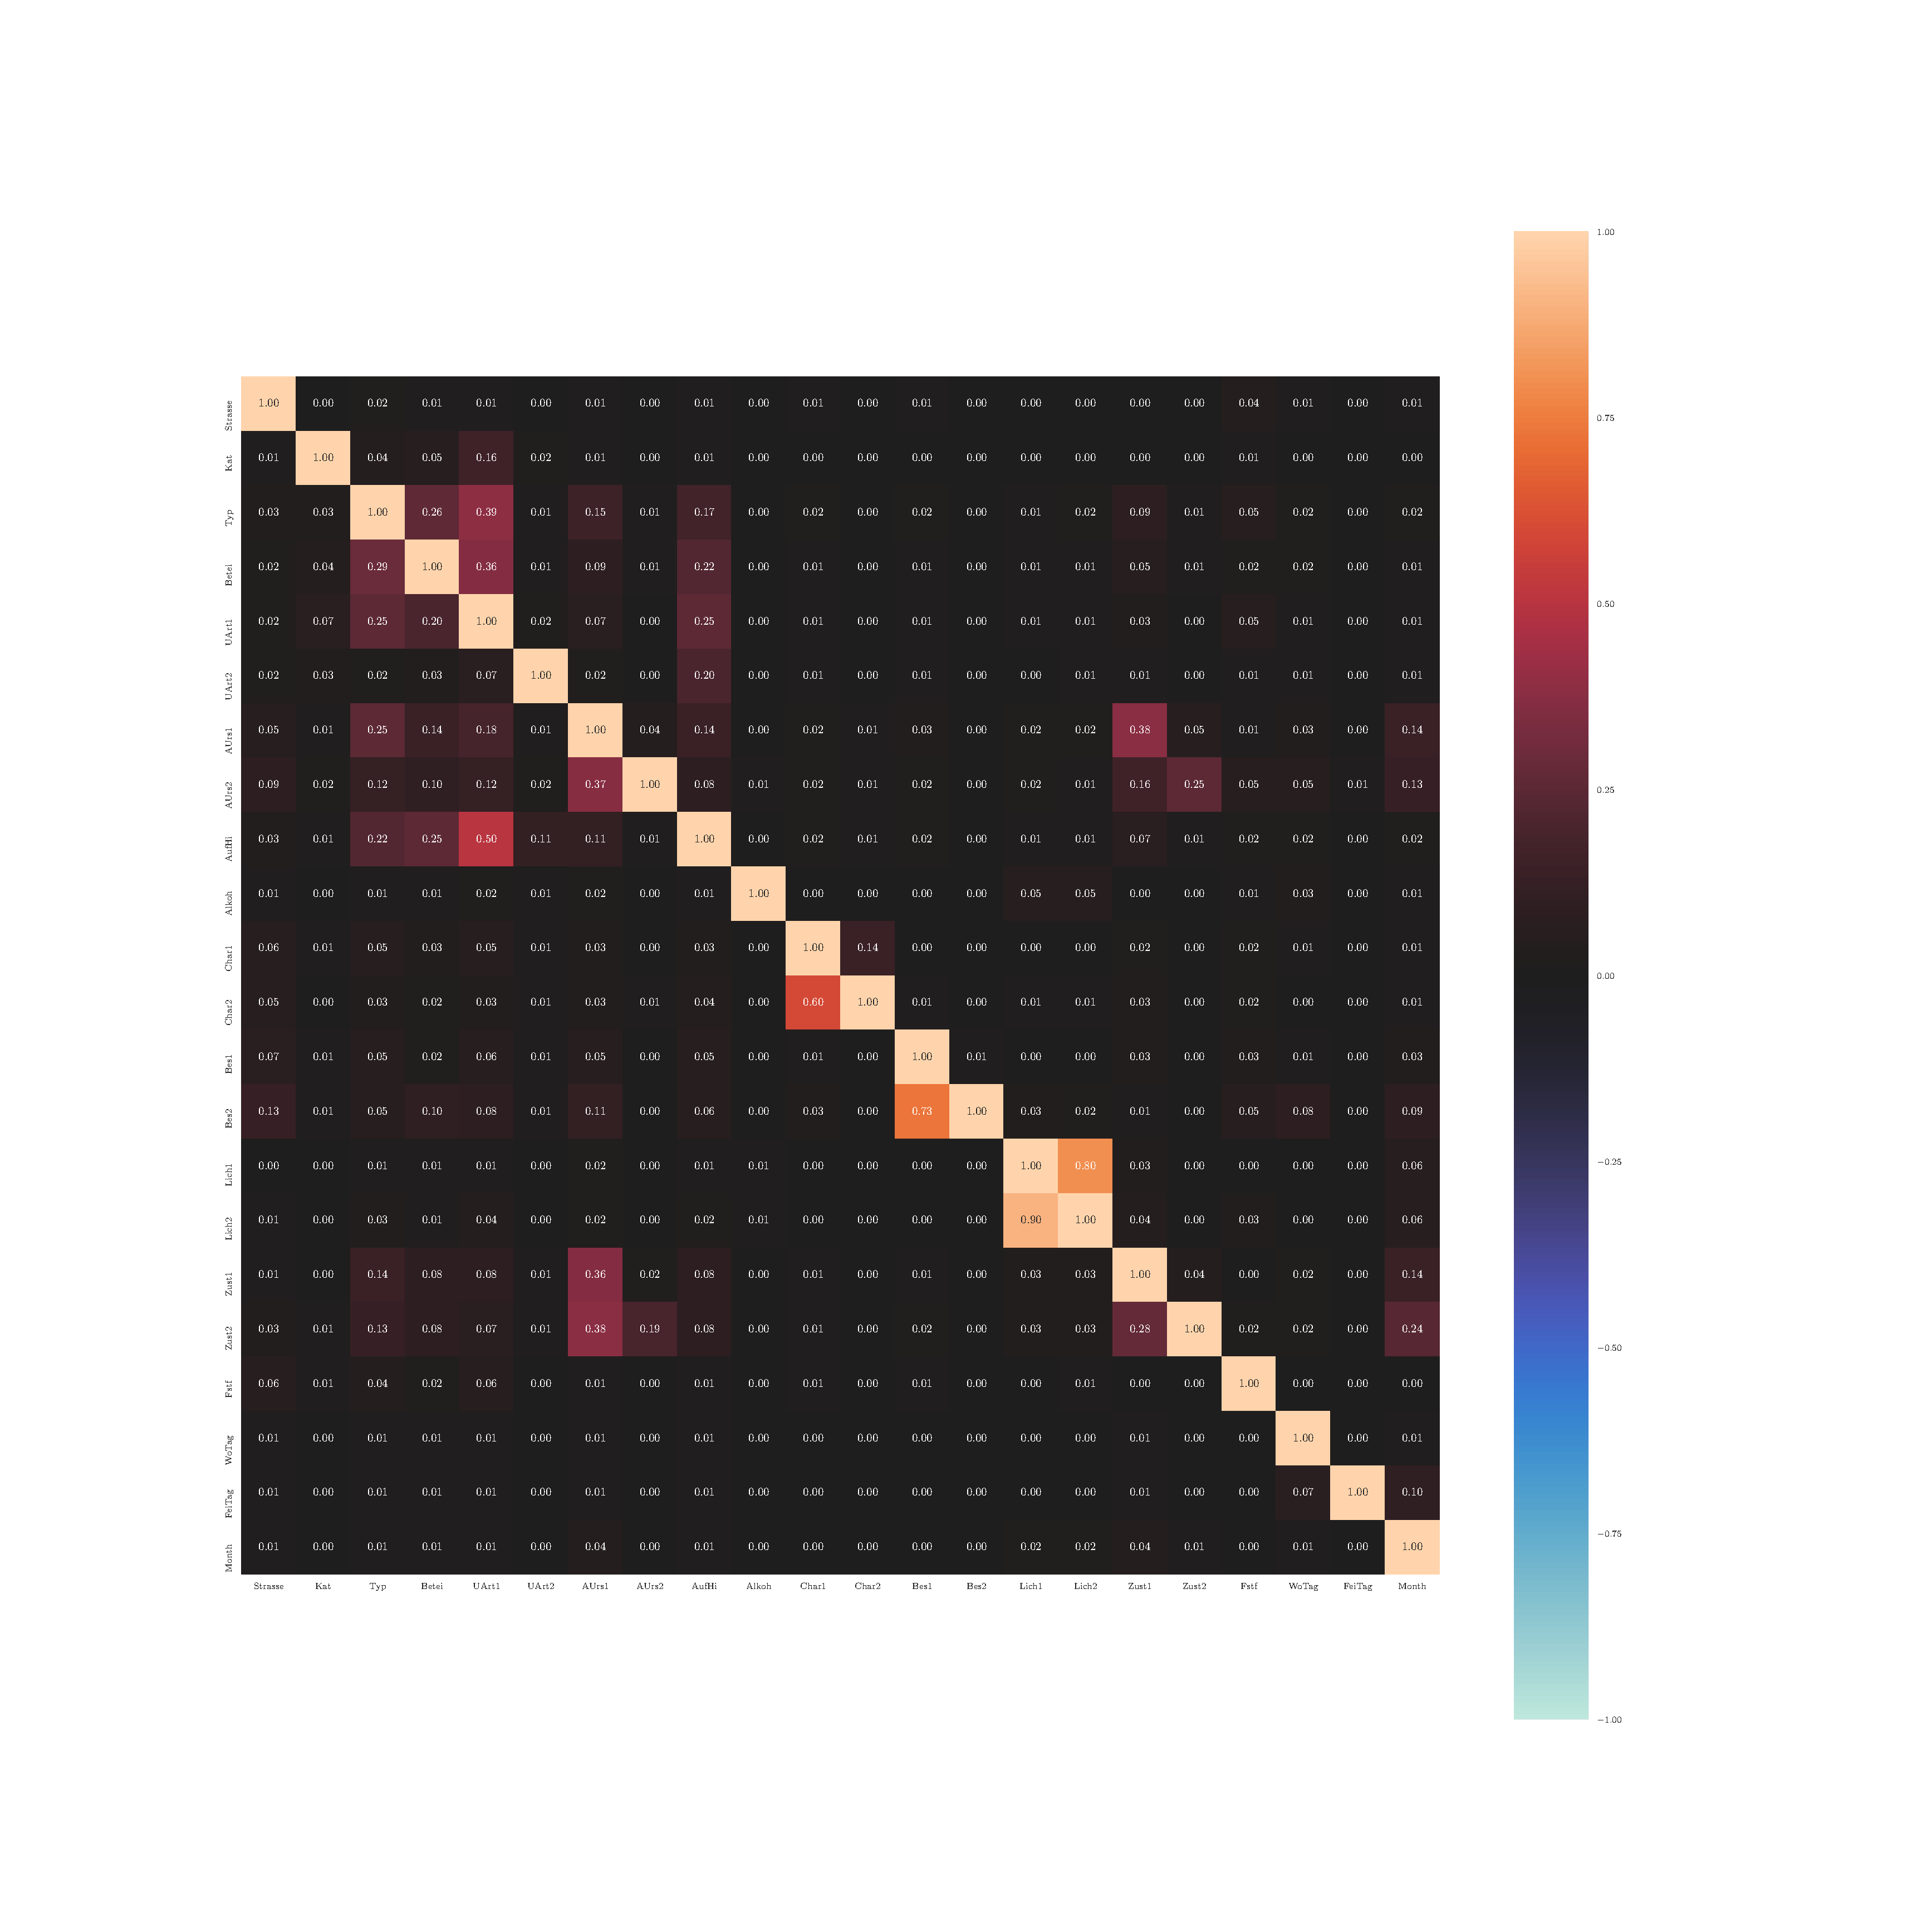
\includegraphics[scale=0.4]{../CorrAnalysis/data/BAYSIS/01_dataset/plots/baysis_dataset_corr_theils}
	\caption{Correlation matrix for BAYSIS dataset, with Theil's $U$}
	\label{img:appendix_correlation_matrix_dataset_theils}
\end{figure}
\restoregeometry

\newgeometry{left=1cm,right=1cm,top=1cm}
\begin{sidewaystable} % <-- HERE
\tiny
\setlength{\tabcolsep}{4pt}
\centering
\begin{tabular}{lrrrrrrrrrrrrrrrrrrrr}
\toprule
{} &  Strasse &  Kat &  Typ &  Betei &  UArt1 &  UArt2 &  AUrs1 &  AUrs2 &  AufHi &  Alkoh &  Char1 &  Char2 &  Lich1 &  Lich2 &  Zust1 &  Zust2 &  Fstf &  WoTag &  FeiTag &  Month \\
\midrule
Strasse &     1.00 & 0.07 & 0.11 &   0.08 &   0.09 &   0.05 &   0.07 &   0.04 &   0.08 &   0.07 &   0.12 &   0.10 &   0.05 &   0.06 &   0.10 &   0.06 &  0.15 &   0.09 &    0.05 &   0.05 \\
Kat     &     0.07 & 1.00 & 0.16 &   0.18 &   0.31 &   0.10 &   0.08 &   0.05 &   0.12 &   0.02 &   0.05 &   0.03 &   0.02 &   0.04 &   0.05 &   0.02 &  0.08 &   0.04 &    0.03 &   0.05 \\
Typ     &     0.11 & 0.16 & 1.00 &   0.31 &   0.56 &   0.06 &   0.26 &   0.06 &   0.25 &   0.06 &   0.15 &   0.09 &   0.09 &   0.20 &   0.33 &   0.12 &  0.16 &   0.08 &    0.05 &   0.09 \\
Betei   &     0.08 & 0.18 & 0.31 &   1.00 &   0.28 &   0.06 &   0.14 &   0.20 &   0.24 &   0.04 &   0.07 &   0.07 &   0.09 &   0.09 &   0.25 &   0.10 &  0.08 &   0.07 &    0.06 &   0.06 \\
UArt1   &     0.09 & 0.31 & 0.56 &   0.28 &   1.00 &   0.08 &   0.21 &   0.05 &   0.32 &   0.05 &   0.14 &   0.09 &   0.10 &   0.22 &   0.25 &   0.09 &  0.16 &   0.08 &    0.05 &   0.06 \\
UArt2   &     0.05 & 0.10 & 0.06 &   0.06 &   0.08 &   1.00 &   0.06 &   0.03 &   0.15 &   0.04 &   0.03 &   0.05 &   0.03 &   0.05 &   0.08 &   0.04 &  0.04 &   0.04 &    0.01 &   0.04 \\
AUrs1   &     0.07 & 0.08 & 0.26 &   0.14 &   0.21 &   0.06 &   1.00 &   0.20 &   0.16 &   0.05 &   0.08 &   0.09 &   0.12 &   0.13 &   0.66 &   0.77 &  0.05 &   0.09 &    0.04 &   0.15 \\
AUrs2   &     0.04 & 0.05 & 0.06 &   0.20 &   0.05 &   0.03 &   0.20 &   1.00 &   0.06 &   0.04 &   0.03 &   0.06 &   0.04 &   0.03 &   0.12 &   0.33 &  0.03 &   0.03 &    0.03 &   0.05 \\
AufHi   &     0.08 & 0.12 & 0.25 &   0.24 &   0.32 &   0.15 &   0.16 &   0.06 &   1.00 &   0.04 &   0.08 &   0.10 &   0.08 &   0.10 &   0.25 &   0.09 &  0.06 &   0.07 &    0.04 &   0.06 \\
Alkoh   &     0.07 & 0.02 & 0.06 &   0.04 &   0.05 &   0.04 &   0.05 &   0.04 &   0.04 &   1.00 &   0.02 &   0.00 &   0.11 &   0.11 &   0.03 &   0.01 &  0.05 &   0.08 &    0.01 &   0.05 \\
Char1   &     0.12 & 0.05 & 0.15 &   0.07 &   0.14 &   0.03 &   0.08 &   0.03 &   0.08 &   0.02 &   1.00 &   0.58 &   0.04 &   0.05 &   0.10 &   0.03 &  0.06 &   0.03 &    0.02 &   0.04 \\
Char2   &     0.10 & 0.03 & 0.09 &   0.07 &   0.09 &   0.05 &   0.09 &   0.06 &   0.10 &   0.00 &   0.58 &   1.00 &   0.04 &   0.04 &   0.08 &   0.03 &  0.08 &   0.03 &    0.02 &   0.04 \\
Lich1   &     0.05 & 0.02 & 0.09 &   0.09 &   0.10 &   0.03 &   0.12 &   0.04 &   0.08 &   0.11 &   0.04 &   0.04 &   1.00 &   0.71 &   0.16 &   0.06 &  0.05 &   0.04 &    0.03 &   0.21 \\
Lich2   &     0.06 & 0.04 & 0.20 &   0.09 &   0.22 &   0.05 &   0.13 &   0.03 &   0.10 &   0.11 &   0.05 &   0.04 &   0.71 &   1.00 &   0.16 &   0.06 &  0.17 &   0.04 &    0.03 &   0.20 \\
Zust1   &     0.10 & 0.05 & 0.33 &   0.25 &   0.25 &   0.08 &   0.66 &   0.12 &   0.25 &   0.03 &   0.10 &   0.08 &   0.16 &   0.16 &   1.00 &   0.17 &  0.06 &   0.12 &    0.05 &   0.37 \\
Zust2   &     0.06 & 0.02 & 0.12 &   0.10 &   0.09 &   0.04 &   0.77 &   0.33 &   0.09 &   0.01 &   0.03 &   0.03 &   0.06 &   0.06 &   0.17 &   1.00 &  0.05 &   0.06 &    0.02 &   0.17 \\
Fstf    &     0.15 & 0.08 & 0.16 &   0.08 &   0.16 &   0.04 &   0.05 &   0.03 &   0.06 &   0.05 &   0.06 &   0.08 &   0.05 &   0.17 &   0.06 &   0.05 &  1.00 &   0.03 &    0.02 &   0.04 \\
WoTag   &     0.09 & 0.04 & 0.08 &   0.07 &   0.08 &   0.04 &   0.09 &   0.03 &   0.07 &   0.08 &   0.03 &   0.03 &   0.04 &   0.04 &   0.12 &   0.06 &  0.03 &   1.00 &    0.13 &   0.09 \\
FeiTag  &     0.05 & 0.03 & 0.05 &   0.06 &   0.05 &   0.01 &   0.04 &   0.03 &   0.04 &   0.01 &   0.02 &   0.02 &   0.03 &   0.03 &   0.05 &   0.02 &  0.02 &   0.13 &    1.00 &   0.13 \\
Month   &     0.05 & 0.05 & 0.09 &   0.06 &   0.06 &   0.04 &   0.15 &   0.05 &   0.06 &   0.05 &   0.04 &   0.04 &   0.21 &   0.20 &   0.37 &   0.17 &  0.04 &   0.09 &    0.13 &   1.00 \\
\bottomrule
\end{tabular}

\caption{Correlation matrix for BAYSIS dataset, with Cramer's $V$}
\end{sidewaystable} % <-- HERE

\begin{sidewaystable} % <-- HERE
\tiny
\setlength{\tabcolsep}{4pt}
\centering
\begin{tabular}{lrrrrrrrrrrrrrrrrrrrrrr}
\toprule
{} &  Strasse &  Kat &  Typ &  Betei &  UArt1 &  UArt2 &  AUrs1 &  AUrs2 &  AufHi &  Alkoh &  Char1 &  Char2 &  Bes1 &  Bes2 &  Lich1 &  Lich2 &  Zust1 &  Zust2 &  Fstf &  WoTag &  FeiTag &  Month \\
\midrule
Strasse &     1.00 & 0.00 & 0.02 &   0.01 &   0.01 &   0.00 &   0.01 &   0.00 &   0.01 &   0.00 &   0.01 &   0.00 &  0.01 &  0.00 &   0.00 &   0.00 &   0.00 &   0.00 &  0.04 &   0.01 &    0.00 &   0.01 \\
Kat     &     0.01 & 1.00 & 0.04 &   0.05 &   0.16 &   0.02 &   0.01 &   0.00 &   0.01 &   0.00 &   0.00 &   0.00 &  0.00 &  0.00 &   0.00 &   0.00 &   0.00 &   0.00 &  0.01 &   0.00 &    0.00 &   0.00 \\
Typ     &     0.03 & 0.03 & 1.00 &   0.26 &   0.39 &   0.01 &   0.15 &   0.01 &   0.17 &   0.00 &   0.02 &   0.00 &  0.02 &  0.00 &   0.01 &   0.02 &   0.09 &   0.01 &  0.05 &   0.02 &    0.00 &   0.02 \\
Betei   &     0.02 & 0.04 & 0.29 &   1.00 &   0.36 &   0.01 &   0.09 &   0.01 &   0.22 &   0.00 &   0.01 &   0.00 &  0.01 &  0.00 &   0.01 &   0.01 &   0.05 &   0.01 &  0.02 &   0.02 &    0.00 &   0.01 \\
UArt1   &     0.02 & 0.07 & 0.25 &   0.20 &   1.00 &   0.02 &   0.07 &   0.00 &   0.25 &   0.00 &   0.01 &   0.00 &  0.01 &  0.00 &   0.01 &   0.01 &   0.03 &   0.00 &  0.05 &   0.01 &    0.00 &   0.01 \\
UArt2   &     0.02 & 0.03 & 0.02 &   0.03 &   0.07 &   1.00 &   0.02 &   0.00 &   0.20 &   0.00 &   0.01 &   0.00 &  0.01 &  0.00 &   0.00 &   0.01 &   0.01 &   0.00 &  0.01 &   0.01 &    0.00 &   0.01 \\
AUrs1   &     0.05 & 0.01 & 0.25 &   0.14 &   0.18 &   0.01 &   1.00 &   0.04 &   0.14 &   0.00 &   0.02 &   0.01 &  0.03 &  0.00 &   0.02 &   0.02 &   0.38 &   0.05 &  0.01 &   0.03 &    0.00 &   0.14 \\
AUrs2   &     0.09 & 0.02 & 0.12 &   0.10 &   0.12 &   0.02 &   0.37 &   1.00 &   0.08 &   0.01 &   0.02 &   0.01 &  0.02 &  0.00 &   0.02 &   0.01 &   0.16 &   0.25 &  0.05 &   0.05 &    0.01 &   0.13 \\
AufHi   &     0.03 & 0.01 & 0.22 &   0.25 &   0.50 &   0.11 &   0.11 &   0.01 &   1.00 &   0.00 &   0.02 &   0.01 &  0.02 &  0.00 &   0.01 &   0.01 &   0.07 &   0.01 &  0.02 &   0.02 &    0.00 &   0.02 \\
Alkoh   &     0.01 & 0.00 & 0.01 &   0.01 &   0.02 &   0.01 &   0.02 &   0.00 &   0.01 &   1.00 &   0.00 &   0.00 &  0.00 &  0.00 &   0.05 &   0.05 &   0.00 &   0.00 &  0.01 &   0.03 &    0.00 &   0.01 \\
Char1   &     0.06 & 0.01 & 0.05 &   0.03 &   0.05 &   0.01 &   0.03 &   0.00 &   0.03 &   0.00 &   1.00 &   0.14 &  0.00 &  0.00 &   0.00 &   0.00 &   0.02 &   0.00 &  0.02 &   0.01 &    0.00 &   0.01 \\
Char2   &     0.05 & 0.00 & 0.03 &   0.02 &   0.03 &   0.01 &   0.03 &   0.01 &   0.04 &   0.00 &   0.60 &   1.00 &  0.01 &  0.00 &   0.01 &   0.01 &   0.03 &   0.00 &  0.02 &   0.00 &    0.00 &   0.01 \\
Bes1    &     0.07 & 0.01 & 0.05 &   0.02 &   0.06 &   0.01 &   0.05 &   0.00 &   0.05 &   0.00 &   0.01 &   0.00 &  1.00 &  0.01 &   0.00 &   0.00 &   0.03 &   0.00 &  0.03 &   0.01 &    0.00 &   0.03 \\
Bes2    &     0.13 & 0.01 & 0.05 &   0.10 &   0.08 &   0.01 &   0.11 &   0.00 &   0.06 &   0.00 &   0.03 &   0.00 &  0.73 &  1.00 &   0.03 &   0.02 &   0.01 &   0.00 &  0.05 &   0.08 &    0.00 &   0.09 \\
Lich1   &     0.00 & 0.00 & 0.01 &   0.01 &   0.01 &   0.00 &   0.02 &   0.00 &   0.01 &   0.01 &   0.00 &   0.00 &  0.00 &  0.00 &   1.00 &   0.80 &   0.03 &   0.00 &  0.00 &   0.00 &    0.00 &   0.06 \\
Lich2   &     0.01 & 0.00 & 0.03 &   0.01 &   0.04 &   0.00 &   0.02 &   0.00 &   0.02 &   0.01 &   0.00 &   0.00 &  0.00 &  0.00 &   0.90 &   1.00 &   0.04 &   0.00 &  0.03 &   0.00 &    0.00 &   0.06 \\
Zust1   &     0.01 & 0.00 & 0.14 &   0.08 &   0.08 &   0.01 &   0.36 &   0.02 &   0.08 &   0.00 &   0.01 &   0.00 &  0.01 &  0.00 &   0.03 &   0.03 &   1.00 &   0.04 &  0.00 &   0.02 &    0.00 &   0.14 \\
Zust2   &     0.03 & 0.01 & 0.13 &   0.08 &   0.07 &   0.01 &   0.38 &   0.19 &   0.08 &   0.00 &   0.01 &   0.00 &  0.02 &  0.00 &   0.03 &   0.03 &   0.28 &   1.00 &  0.02 &   0.02 &    0.00 &   0.24 \\
Fstf    &     0.06 & 0.01 & 0.04 &   0.02 &   0.06 &   0.00 &   0.01 &   0.00 &   0.01 &   0.00 &   0.01 &   0.00 &  0.01 &  0.00 &   0.00 &   0.01 &   0.00 &   0.00 &  1.00 &   0.00 &    0.00 &   0.00 \\
WoTag   &     0.01 & 0.00 & 0.01 &   0.01 &   0.01 &   0.00 &   0.01 &   0.00 &   0.01 &   0.00 &   0.00 &   0.00 &  0.00 &  0.00 &   0.00 &   0.00 &   0.01 &   0.00 &  0.00 &   1.00 &    0.00 &   0.01 \\
FeiTag  &     0.01 & 0.00 & 0.01 &   0.01 &   0.01 &   0.00 &   0.01 &   0.00 &   0.01 &   0.00 &   0.00 &   0.00 &  0.00 &  0.00 &   0.00 &   0.00 &   0.01 &   0.00 &  0.00 &   0.07 &    1.00 &   0.10 \\
Month   &     0.01 & 0.00 & 0.01 &   0.01 &   0.01 &   0.00 &   0.04 &   0.00 &   0.01 &   0.00 &   0.00 &   0.00 &  0.00 &  0.00 &   0.02 &   0.02 &   0.04 &   0.01 &  0.00 &   0.01 &    0.00 &   1.00 \\
\bottomrule
\end{tabular}

\caption{Correlation matrix for BAYSIS dataset, with Theil's $U$}
\end{sidewaystable} % <-- HERE

\begin{sidewaystable} % <-- HERE
\tiny
\setlength{\tabcolsep}{4pt}
\centering
\begin{tabular}{lrrrrrrrrrrrrrrrrrrrrrrr}
\toprule
{} &  Strasse &   Kat &   Typ &  Betei &  UArt1 &  UArt2 &  AUrs1 &  AUrs2 &  AufHi &  Alkoh &  Char1 &  Char2 &  Bes1 &  Bes2 &  Lich1 &  Lich2 &  Zust1 &  Zust2 &  Fstf &  StrklVu &  WoTag &  FeiTag &  Month \\
\midrule
Strasse &      nan & 0.000 & 0.000 &  0.000 &  0.000 &  0.000 &  0.000 &  0.871 &  0.000 &  0.000 &  0.000 &  0.000 & 0.000 & 0.357 &  0.165 &  0.000 &  0.000 &  0.006 & 0.000 &    0.870 &  0.000 &   0.073 &  0.002 \\
Kat     &    0.000 &   nan & 0.000 &  0.000 &  0.000 &  0.000 &  0.000 &  0.000 &  0.000 &  0.225 &  0.000 &  0.058 & 0.000 & 0.754 &  0.260 &  0.000 &  0.000 &  0.068 & 0.000 &    0.760 &  0.000 &   0.069 &  0.000 \\
Typ     &    0.000 & 0.000 &   nan &  0.000 &  0.000 &  0.000 &  0.000 &  0.000 &  0.000 &  0.000 &  0.000 &  0.000 & 0.000 & 0.691 &  0.000 &  0.000 &  0.000 &  0.000 & 0.000 &    0.000 &  0.000 &   0.000 &  0.000 \\
Betei   &    0.000 & 0.000 & 0.000 &    nan &  0.000 &  0.000 &  0.000 &  0.000 &  0.000 &  0.463 &  0.000 &  0.000 & 0.000 & 0.208 &  0.000 &  0.000 &  0.000 &  0.000 & 0.000 &    1.000 &  0.000 &   0.000 &  0.000 \\
UArt1   &    0.000 & 0.000 & 0.000 &  0.000 &    nan &  0.000 &  0.000 &  0.000 &  0.000 &  0.000 &  0.000 &  0.000 & 0.000 & 0.534 &  0.000 &  0.000 &  0.000 &  0.000 & 0.000 &    0.000 &  0.000 &   0.001 &  0.000 \\
UArt2   &    0.000 & 0.000 & 0.000 &  0.000 &  0.000 &    nan &  0.000 &  0.045 &  0.000 &  0.017 &  0.043 &  0.001 & 0.000 & 1.000 &  0.122 &  0.001 &  0.000 &  0.002 & 0.000 &    1.000 &  0.016 &   0.998 &  0.054 \\
AUrs1   &    0.000 & 0.000 & 0.000 &  0.000 &  0.000 &  0.000 &    nan &  0.000 &  0.000 &  0.157 &  0.000 &  0.000 & 0.000 & 0.000 &  0.000 &  0.000 &  0.000 &  0.000 & 0.002 &    1.000 &  0.000 &   0.386 &  0.000 \\
AUrs2   &    0.871 & 0.000 & 0.000 &  0.000 &  0.000 &  0.045 &  0.000 &    nan &  0.000 &  0.070 &  0.130 &  0.000 & 0.001 & 1.000 &  0.028 &  0.647 &  0.000 &  0.000 & 0.247 &    1.000 &  0.100 &   0.199 &  0.000 \\
AufHi   &    0.000 & 0.000 & 0.000 &  0.000 &  0.000 &  0.000 &  0.000 &  0.000 &    nan &  0.026 &  0.000 &  0.000 & 0.000 & 0.844 &  0.000 &  0.000 &  0.000 &  0.000 & 0.000 &    0.798 &  0.000 &   0.066 &  0.000 \\
Alkoh   &    0.000 & 0.225 & 0.000 &  0.463 &  0.000 &  0.017 &  0.157 &  0.070 &  0.026 &    nan &  0.689 &  0.754 & 0.660 & 0.371 &  0.000 &  0.000 &  0.035 &  0.745 & 0.004 &    0.623 &  0.000 &   0.279 &  0.017 \\
Char1   &    0.000 & 0.000 & 0.000 &  0.000 &  0.000 &  0.043 &  0.000 &  0.130 &  0.000 &  0.689 &    nan &  0.000 & 0.000 & 0.475 &  0.000 &  0.000 &  0.000 &  0.017 & 0.000 &    0.716 &  0.007 &   0.415 &  0.084 \\
Char2   &    0.000 & 0.058 & 0.000 &  0.000 &  0.000 &  0.001 &  0.000 &  0.000 &  0.000 &  0.754 &  0.000 &    nan & 0.000 & 0.443 &  0.001 &  0.000 &  0.000 &  0.012 & 0.000 &    0.574 &  0.250 &   0.020 &  0.075 \\
Bes1    &    0.000 & 0.000 & 0.000 &  0.000 &  0.000 &  0.000 &  0.000 &  0.001 &  0.000 &  0.660 &  0.000 &  0.000 &   nan & 0.000 &  0.005 &  0.000 &  0.000 &  0.000 & 0.000 &    0.581 &  0.000 &   0.678 &  0.000 \\
Bes2    &    0.357 & 0.754 & 0.691 &  0.208 &  0.534 &  1.000 &  0.000 &  1.000 &  0.844 &  0.371 &  0.475 &  0.443 & 0.000 &   nan &  0.133 &  0.263 &  0.806 &  0.930 & 0.718 &    0.986 &  0.453 &   0.387 &  0.605 \\
Lich1   &    0.165 & 0.260 & 0.000 &  0.000 &  0.000 &  0.122 &  0.000 &  0.028 &  0.000 &  0.000 &  0.000 &  0.001 & 0.005 & 0.133 &    nan &  0.000 &  0.000 &  0.000 & 0.000 &    0.158 &  0.002 &   0.015 &  0.000 \\
Lich2   &    0.000 & 0.000 & 0.000 &  0.000 &  0.000 &  0.001 &  0.000 &  0.647 &  0.000 &  0.000 &  0.000 &  0.000 & 0.000 & 0.263 &  0.000 &    nan &  0.000 &  0.000 & 0.000 &    0.000 &  0.001 &   0.033 &  0.000 \\
Zust1   &    0.000 & 0.000 & 0.000 &  0.000 &  0.000 &  0.000 &  0.000 &  0.000 &  0.000 &  0.035 &  0.000 &  0.000 & 0.000 & 0.806 &  0.000 &  0.000 &    nan &  0.000 & 0.000 &    0.763 &  0.000 &   0.000 &  0.000 \\
Zust2   &    0.006 & 0.068 & 0.000 &  0.000 &  0.000 &  0.002 &  0.000 &  0.000 &  0.000 &  0.745 &  0.017 &  0.012 & 0.000 & 0.930 &  0.000 &  0.000 &  0.000 &    nan & 0.000 &    0.995 &  0.000 &   0.125 &  0.000 \\
Fstf    &    0.000 & 0.000 & 0.000 &  0.000 &  0.000 &  0.000 &  0.002 &  0.247 &  0.000 &  0.004 &  0.000 &  0.000 & 0.000 & 0.718 &  0.000 &  0.000 &  0.000 &  0.000 &   nan &    0.000 &  0.033 &   0.660 &  0.081 \\
StrklVu &    0.870 & 0.760 & 0.000 &  1.000 &  0.000 &  1.000 &  1.000 &  1.000 &  0.798 &  0.623 &  0.716 &  0.574 & 0.581 & 0.986 &  0.158 &  0.000 &  0.763 &  0.995 & 0.000 &      nan &  0.249 &   0.055 &  0.166 \\
WoTag   &    0.000 & 0.000 & 0.000 &  0.000 &  0.000 &  0.016 &  0.000 &  0.100 &  0.000 &  0.000 &  0.007 &  0.250 & 0.000 & 0.453 &  0.002 &  0.001 &  0.000 &  0.000 & 0.033 &    0.249 &    nan &   0.000 &  0.000 \\
FeiTag  &    0.073 & 0.069 & 0.000 &  0.000 &  0.001 &  0.998 &  0.386 &  0.199 &  0.066 &  0.279 &  0.415 &  0.020 & 0.678 & 0.387 &  0.015 &  0.033 &  0.000 &  0.125 & 0.660 &    0.055 &  0.000 &     nan &  0.000 \\
Month   &    0.002 & 0.000 & 0.000 &  0.000 &  0.000 &  0.054 &  0.000 &  0.000 &  0.000 &  0.017 &  0.084 &  0.075 & 0.000 & 0.605 &  0.000 &  0.000 &  0.000 &  0.000 & 0.081 &    0.166 &  0.000 &   0.000 &    nan \\
\bottomrule
\end{tabular}

\caption{Significancy matrix for BAYSIS dataset}
\end{sidewaystable} % <-- HERE
\restoregeometry


\chapter{ArbIS Dataset Figures}
\tocless\section{Figure Name}
\label{appendix_TODO}

%\tocless\section{}
\newgeometry{left=1cm,right=1cm,top=1cm}
\label{appendix_baysis_dataset_corr_theils}
\begin{figure}[h]
	\centering
	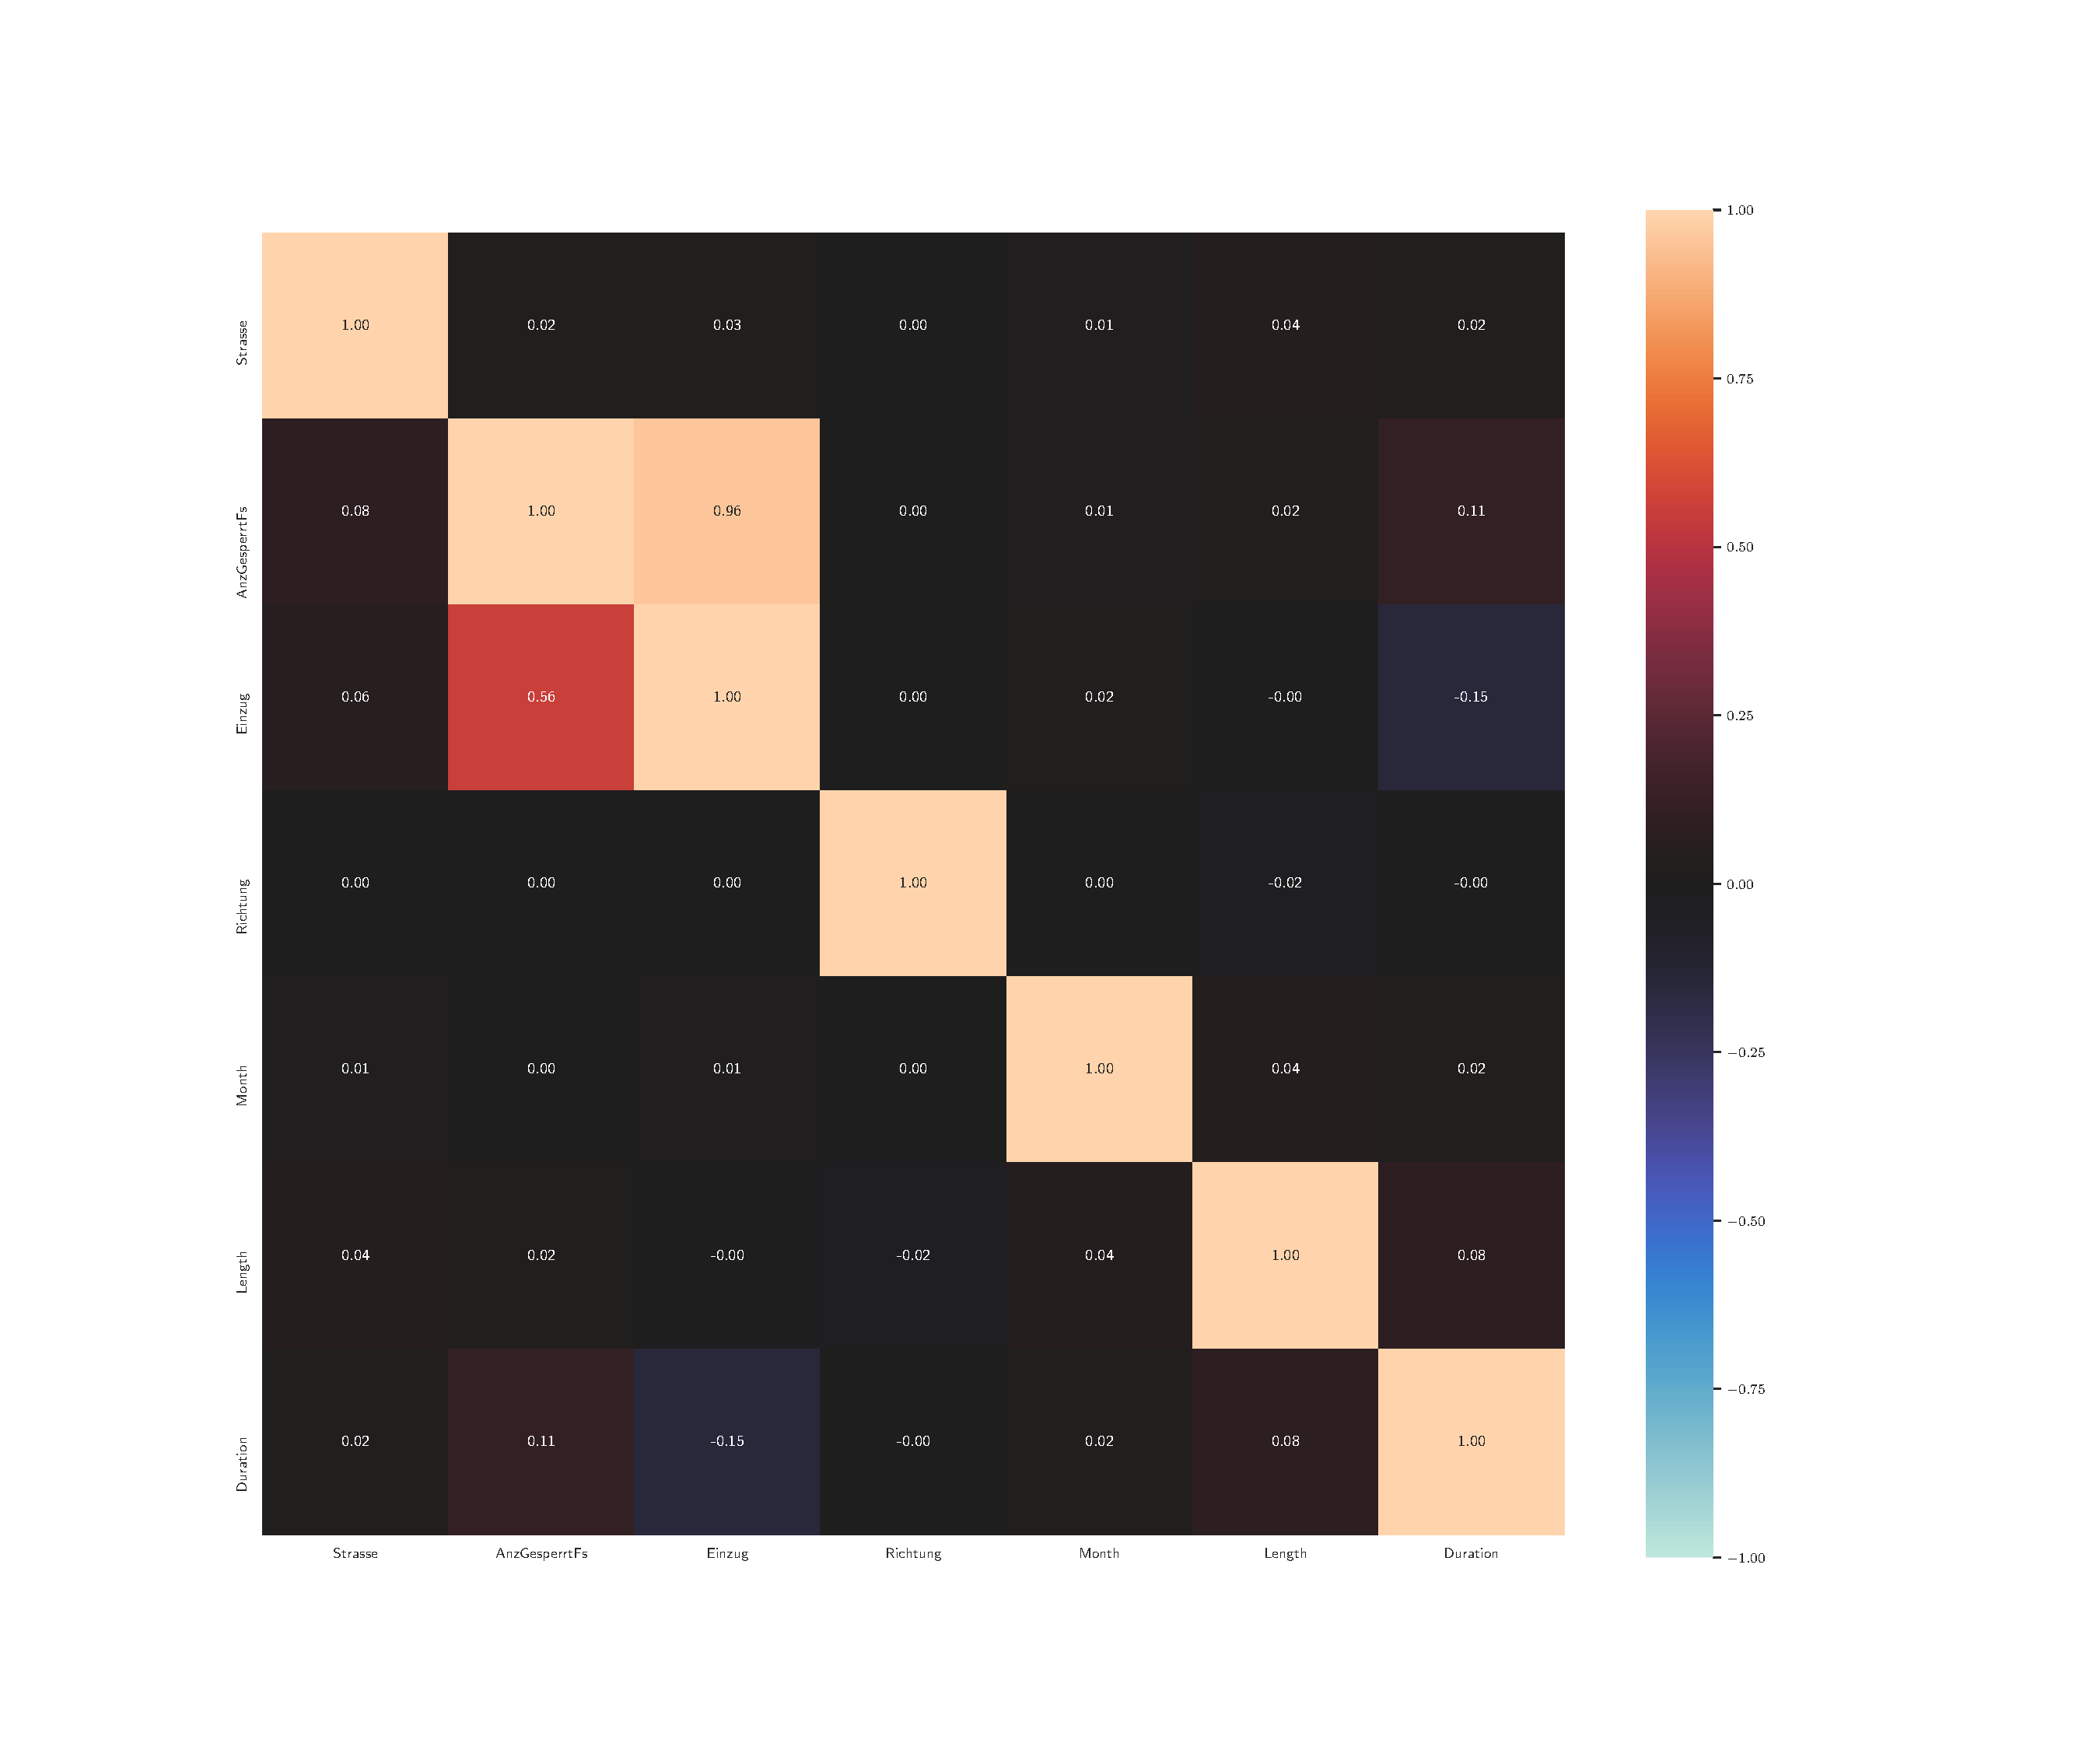
\includegraphics[scale=0.8]{../CorrAnalysis/data/ArbIS/01_dataset/plots/arbis_dataset_corr_theils}
	\caption{Correlation matrix for ArbIS dataset, with Theil's $U$}
	\label{img:appendix_correlation_matrix_dataset_theils}
\end{figure}
\restoregeometry

\newgeometry{left=1cm,right=1cm,top=1cm}
\begin{table}
\setlength{\tabcolsep}{4pt}
\centering
\begin{tabular}{lrrrrrrr}
\toprule
{} &  Strasse &  AnzGesperrtFs &  Einzug &  Richtung &  Month &  Length &  Duration \\
\midrule
Strasse       &     1.00 &           0.16 &    0.17 &      0.05 &   0.06 &    0.04 &      0.02 \\
AnzGesperrtFs &     0.16 &           1.00 &    0.50 &      0.00 &   0.06 &    0.02 &      0.11 \\
Einzug        &     0.17 &           0.50 &    1.00 &      0.02 &   0.11 &   -0.00 &     -0.15 \\
Richtung      &     0.05 &           0.00 &    0.02 &      1.00 &   0.03 &   -0.02 &     -0.00 \\
Month         &     0.06 &           0.06 &    0.11 &      0.03 &   1.00 &    0.04 &      0.02 \\
Length        &     0.04 &           0.02 &   -0.00 &     -0.02 &   0.04 &    1.00 &      0.08 \\
Duration      &     0.02 &           0.11 &   -0.15 &     -0.00 &   0.02 &    0.08 &      1.00 \\
\bottomrule
\end{tabular}

\caption{Correlation matrix for ArbIS dataset, with Cramer's $V$}
\end{table} % <-- HERE

\begin{table}
\setlength{\tabcolsep}{4pt}
\centering
\begin{tabular}{lrrrrrrr}
\toprule
{} &  Strasse &  AnzGesperrtFs &  Einzug &  Richtung &  Month &  Length &  Duration \\
\midrule
Strasse       &     1.00 &           0.02 &    0.03 &      0.00 &   0.01 &    0.04 &      0.02 \\
AnzGesperrtFs &     0.08 &           1.00 &    0.96 &      0.00 &   0.01 &    0.02 &      0.11 \\
Einzug        &     0.06 &           0.56 &    1.00 &      0.00 &   0.02 &   -0.00 &     -0.15 \\
Richtung      &     0.00 &           0.00 &    0.00 &      1.00 &   0.00 &   -0.02 &     -0.00 \\
Month         &     0.01 &           0.00 &    0.01 &      0.00 &   1.00 &    0.04 &      0.02 \\
Length        &     0.04 &           0.02 &   -0.00 &     -0.02 &   0.04 &    1.00 &      0.08 \\
Duration      &     0.02 &           0.11 &   -0.15 &     -0.00 &   0.02 &    0.08 &      1.00 \\
\bottomrule
\end{tabular}

\caption{Correlation matrix for ArbIS dataset, with Theil's $U$}
\end{table} % <-- HERE

\begin{table}
\setlength{\tabcolsep}{4pt}
\centering
\begin{tabular}{lrrrrrrr}
\toprule
{} &  Strasse &  AnzGesperrtFs &  Einzug &  Richtung &  Length &  Duration &  Month \\
\midrule
Strasse       &      NaN &         0.0000 &  0.0000 &    0.0000 &  0.0000 &    0.0000 &    0.0 \\
AnzGesperrtFs &      0.0 &            NaN &  0.0000 &    0.2547 &  0.0000 &    0.0000 &    0.0 \\
Einzug        &      0.0 &         0.0000 &     NaN &    0.0000 &  0.0006 &    0.0000 &    0.0 \\
Richtung      &      0.0 &         0.2547 &  0.0000 &       NaN &  0.0000 &    0.0489 &    0.0 \\
Length        &      0.0 &         0.0000 &  0.0006 &    0.0000 &     NaN &    0.0000 &    0.0 \\
Duration      &      0.0 &         0.0000 &  0.0000 &    0.0489 &  0.0000 &       NaN &    0.0 \\
Month         &      0.0 &         0.0000 &  0.0000 &    0.0000 &  0.0000 &    0.0000 &    NaN \\
\bottomrule
\end{tabular}

\caption{Significancy matrix for ArbIS dataset}
\end{table} % <-- HERE
\restoregeometry

\chapter{Source Code}

\tocless\section{CongstatsClusterAlgorithm}
\label{appendix_TODO}

\newgeometry{left=2cm,top=0.5cm,bottom=0.5cm}
\begingroup
%    \fontsize{4pt}{8pt}\selectfont
%		\lstinputlisting[language=java]{../Code/congestion/clustering/CongstatsClusterAlgorithm.java}
\endgroup
\restoregeometry

\end{appendices}

\pagebreak

\addcontentsline{toc}{chapter}{Declaration of independence}
\chapter*{Declaration of independence}

Erkl\"arung zur Master’s Thesis
\newline \\
Ich versichere hiermit, die vorliegende Arbeit selbst\"andig verfasst und keine anderen Quellen als die angegebenen Quellen und Hilfsmittel benutzt zu haben. Die Arbeit wurde noch nicht anderweitig f\"ur Pr\"ufungszwecke vorgelegt. 
\newline \\ \\ \\
M\"unchen, 15.12.2020 : \hrulefill \newline
\hspace*{0mm}\phantom{M\"unchen, 11.12.2020: } B. Sc. Jakob Erpf

\end{document}
